\documentclass[12pt]{article}
\usepackage[italian]{babel}
\usepackage{graphicx}
\usepackage[section]{placeins}

\title{Metodi Informatici per la Gestione Aziendale}
\author{Giuseppe Facchi}
\date{A.A. 2020-2021}

\begin{document}
\maketitle
\newpage
\tableofcontents
\newpage

\section{Introduzione}
\subsection{Contenuti del corso}
\begin{itemize}
    \item Elementi di Economia e Organizzazione Aziendale
    \item Contabilità e Bilancio
    \item Finanza Aziendale
    \item Marketing Analytics
    \item Recommender systems
          \begin{itemize}
              \item Prediction Version of Problem
              \item Ranking Version of Problem (TOP-K Ranking)
          \end{itemize}
\end{itemize}

\paragraph{Economia}
\begin{itemize}
    \item \textbf{Microeconomia}: Produttori, Consumatori, Mercati
    \item Domanda e Offerta
    \item Incertezza e Comportamento del Consumatore
    \item Platform Economy e Sharing Economy
\end{itemize}

\subsection{Tipi di Economia}
Esistono \textbf{business models} diversi

\subsection{ICT e Business Disruption}
\begin{itemize}
    \item Nelle aziende i processi più importanti diventano mediati digitalmente
    \item Si parla di \textbf{landscape frammentato} e ricomposto in modi imprevedibili
    \item Le piattaforme ICT di relazione/negoziazione iniziano a proporsi per servizi professionali e alla professionali
    \item Nel \textbf{retail} anche la \textbf{customer experience} diventa \textbf{difitally mediated}
\end{itemize}
\newpage
\section{Elementi di economia e org. aziendale}
\subsection{La natura e i fini economi dell'impresa}
\paragraph{Attività economica} L'insieme delle operazioni finalizzate alla produzione, distribuzione o al consumo di \textbf{beni economici}
\paragraph{Beni economici} Beni utili a soddisfare i bisogni delle persone e SCARSI (non illimitati)

\paragraph{}\textit{Non tutti i bisogni delle persone sono affidati a imprese (es. sicurezza e giustizia), esistono però compromessi come la sanità}

\paragraph{} Quando si realizzano queste condizioni:
\begin{itemize}
    \item Esistenza di una \textbf{domanda} e \textbf{offerta}
    \item Esistenza di \textbf{soggetti} in grado di \textbf{offrire} questo \textbf{prodotto} agli acquirenti
    \item \textbf{Acquisizione} e \textbf{organizzazione} dei \textbf{fattori di produzione}
\end{itemize}
Allora la \textbf{progettazione/produzione} e \textbf{vendita} di \textbf{beni e servizi} sono realizzate a una particolare forma di organizzazione umana chiamata \textbf{impresa}.

\paragraph{Prezzi di vendita} Ai prezzi di vendita (accettabili per gli acquirenti) devono corrispondere \textbf{ricavi adeguati} a remunerare i costi di produzione.

\subsection{Gli Istituti Economici}
Quando \textbf{l'attività economica} è svolta attraverso realtà:
\begin{itemize}
    \item \textbf{Organizzate}
    \item \textbf{Durature}
    \item \textbf{Autonome}
\end{itemize}
si è in presenza di \textbf{istituti economici}
\begin{itemize}
    \item Famiglie
    \item Enti no-profit
    \item Amministrazioni pubbliche
    \item \textbf{imprese}
\end{itemize}

\subsubsection{L'istituto "impresa"}
Si caratterizza per la \textbf{specializzazione} in quella prate di \textbf{attività economica} che si manifesta attraverso la produzione e vendita sul \textbf{mercato} di prodotti \textit{(Beni/Servizi)}
\begin{itemize}
    \item \textbf{Combina} e \textbf{Trasforma} le risorse per realizzare prodotti di \textbf{maggior utilità e valore}
    \item Il processo di produzione \textbf{genera ricchezza} poiché \textbf{accresce il valore} (in termini monetizzabili) \textbf{finale dell'output} rispetto all'input
\end{itemize}

\subsection{Oggetto di analisi dell'ec. aziendale}
L'impresa è analizzabile come \textbf{combinazione di fattori produttivi}
\begin{itemize}
    \item \textbf{Lavoro}
    \item \textbf{Capitale}
\end{itemize}

\paragraph{}\textit{La \textbf{proprietà intellettuale} riveste un ruolo decisivo nella generazione del CASH-FLOW di un'azienda $\rightarrow$ \textbf{Immobilizzazioni Immateriali}}
\newline
\newline
L'\textbf{economia aziendale}
\begin{itemize}
    \item \textbf{Rileva}
    \item \textbf{Analizza}
    \item \textbf{Descrive}
\end{itemize}
tutte le \textbf{operazioni} pertinenti alle condizioni di produzione e in generale all'attività economica
\begin{itemize}
    \item Trasformazione Fisico-Tecnica
    \item Negoziazione di beni e servizi
    \item Organizzazione
    \item Rilevazione e informazione
\end{itemize}

\subsection{L'impresa come sistema}
L'impresa è un \textbf{sistema} in quanto è costituita da \textbf{diversi elementi} legati da relazione di \textbf{interdipendenza} e \textbf{combinati} tra loro per il raggiungimento di obiettivi prefissati. L'impresa è un sistema di tipo
\begin{itemize}
    \item \textbf{APERTO}: scambia input e output con l'ambiente in cui opera
    \item \textbf{DINAMICO}: modifica continuamente la sua configurazione
    \item \textbf{COMPLESSO}: ogni attività genera osservazioni di un elevano numero di variabili
    \item \textbf{UNITARIO}: Un corpo organico unico e unico mosso da un fine comune $\rightarrow$ \textit{Sistema decisionale TOP-DOWN}
\end{itemize}

\subsubsection{Sistema Aperto}
L'impresa nel proprio ambiente di riferimento \textbf{interagisce, scambia} continuamente risorse ed energia con altri attori secondo un modello \textbf{input-output}
\begin{itemize}
    \item \textbf{INPUT}: Importazione dall'esterno di fattori di produzione
    \item \textbf{OUTPUT}: Trasformazione dell'input e restituzione all'ambiente in forma di prodotti/servizi
\end{itemize}

\paragraph{}\textit{Esistono anche modelli \textbf{chiusi} (es. closed innovation system) dove esiste un solo input ed hanno una sola via d'uscita verso il mercato (es. Big Pharma) a cui vengono contrapposti sistemi \textbf{aperti} (es. Open Innovation Paradigm)}

\subsubsection{Sistema Dinamico}
Durante l'\textbf{attività ciclica} diu scambio con l'ambiente l'impresa \textbf{modifica costantemente} il suo assetto. Tende ad uno \textbf{stato di equilibrio dinamico} con il suo \textbf{ambiente} e al mutare delle condizioni esterne tende a mutare al suo interno con \textbf{procedure di retroazione} fino ad un nuovo equilibrio.

\subsubsection{Sistema Unitario}
L'impresa deve essere considerata come un corpo \textbf{unico} e \textbf{unito}

\subsection{L'impresa come attore sociale responsabile}
L'impresa si relaziona continuamente con gli \textbf{stakeholders}
\begin{itemize}
    \item Clienti
    \item Organizzazioni civili, politiche, organi legislativi
    \item Organi governativi
    \item Gruppi tutelatori degli interessi dei cittadini/lavoratori
\end{itemize}
La \textbf{responsabilità sociale} dell'impresa intende sottolineare la necessità per l'impresa di tener conto degli \textbf{interessi degli stakeholders} nelle sue scelte/azioni. Le aziende che riescono nell'intento vengono chiamate \textbf{Benefit Companies}

\subsection{Spazio decisionale dell'impresa}
\begin{itemize}
    \item \textbf{Incertezza}: Le decisioni strategiche fanno riferimento ad \textbf{archi temporali lunghi} in cui dominano \textbf{incertezze sui costi} dei fattori di produzione, \textbf{incertezze sui riferimenti amministrativi/istituzionali} e \textbf{incertezze sulla domanda} dei prodotti attuali
    \item \textbf{Diversi interessi da bilanciare}
    \item \textbf{Diversi decisori}: Contrasti tra \textbf{management} e \textbf{azionisti}
\end{itemize}
La comunità locale dove un'impresa industriale ha un grande stabilimento può trovarsi a \textbf{sopportare notevoli esternalità} dovute alla sua presenza
\begin{itemize}
    \item \textbf{Esternalità negative} (es. inquinamento)
    \item \textbf{Esternalità positive} (es. promozione di attività economiche dell'indotto)
\end{itemize}
Esiste anche una consapevolezza nel dover \textbf{gestire la responsabilità sociale (benefit companies)}
\begin{itemize}
    \item Bilancio ambientale
    \item Carte dei valori/Codici di comportamento
    \item Certificazioni sulla qualità
    \item Correttezza nella gestione del personale
\end{itemize}

\subsection{Principi base per il governo delle imprese}

\begin{itemize}
    \item Le \textbf{responsabilità} e il \textbf{potere di governo} spettano a coloro che rappresentano il \textbf{soggetto economico} (coincide spesso con i detentori del capitale sociale)
    \item Il perseguimento esclusivo del proprio interesse non può costituire il principio assoluto che orienta le decisioni del soggetto economico, bisogna infatti \textbf{rispettare le condizioni di equilibrio di medio/lungo termine} tra diverse grandezze economiche e tra gli stakeholders
\end{itemize}
Affinché le imprese possano risultare \textbf{durature} e aspirare al raggiungimento del loro \textbf{fine istituzionale} il \textbf{processo decisionale} del soggetto economico deve svolgersi sul rispetto di \textbf{due principi di governo}
\begin{itemize}
    \item \textbf{Principio di Economicità} che attiene alla natura economica del suo agire
    \item \textbf{Principio del Contemperamento degli Interessi} che fa riferimento al fine per cui l'impresa è stata costituita e opera (non solo il profitto)
\end{itemize}

\paragraph{Rule of Law} Certezza del diritto
\paragraph{Sostenibilità Ambientale} L'impresa deve essere governata seguendo il principio di sostenibilità ambientale
\paragraph{Equal Opportunity Employer} Tutela delle minoranze

\subsection{Il principio di economicità}
Il \textbf{soggetto economico} deve decidere e agire facendo in modo di perseguire per l'impresa:
\begin{itemize}
    \item \textbf{Equilibrio reddituale}: Equilibiro tra i componenti positivi (RICAVI) e negativi (COSTI) $\rightarrow$ Ricavi $>$ Costi
    \item \textbf{Equilibrio monetario}: Le entrate monetarie devono essere sufficienti per far fronte alle loro uscite anche ricorrendo ad una gestione \textit{finanziaria} $\rightarrow$ Entrate $>$ Uscite
    \item \textbf{Livello acettabile} di
          \begin{itemize}
              \item Efficienza (minimizzare gli sprechi)
              \item Flessibilità dei processi produttivi
          \end{itemize}
    \item \textbf{Congruità dei prezzi dei fattori di produzione acquisiti e dei prodotti venduti}
\end{itemize}

L'\textbf{economicità} delle imprese viene valutata attraverso l'analisi dei valori aziendali riferiti a un \textbf{determinato e significativo intervallo temporale} detto \textbf{esercizio}. I valori vengono rilevati mediante \textbf{metodologia contabile} e valutati attraverso il \textbf{bilancio di esercizio}. La \textbf{gestione finanziaria} ha il compito di mantenere un corretto equilibrio tra le diverse fonti di finanziamento dell'impresa e le modalità di impiego dei relativi mezzi finanziari.
L'attività di \textbf{determinazione degli obiettivi economici e di monitoraggio} del loro raggiungimento viene svolta attraverso \textbf{sistemi di programmazione controllo di gestione}.
\newpage
\subsection{L'assetto organizzativo dell'impresa}
L'impresa deve essere
\begin{itemize}
    \item \textbf{ORDINATA} nelle sue attività economiche
    \item \textbf{COORDINATA} nelle sue componenti
    \item \textbf{REGOLATA} nel suo funzionamento
\end{itemize}
L'\textbf{assetto organizzativo} è il risultato della combinazione di varaibili organizzative
\begin{itemize}
    \item \textbf{Struttura organizzativa} che definisce \textit{compiti e responsabilità}
    \item \textbf{Sistemi operativi (o di management)} che regolano e guidano i \textit{comportamenti} delle persone nello \textit{svolgere attività}
\end{itemize}
e ha il compito di \textbf{coniugare} il \textbf{lavoro} delle persone con il \textbf{sistema delle operazioni aziendali elementari} a loro volta combinate in \textbf{attività parziali} (Taylorismo)
\newpage
\section{La struttura organizzativa}
Necessità di
\begin{itemize}
    \item \textbf{Dividere il lavoro} in attività elementari da affidare ai singoli membri per \textit{incrementare la produttività specializzando il personale}
    \item \textbf{Coordinare efficacemente}
\end{itemize}
La struttura organizzativa è la configurazione unitaria e coordinata di
\begin{itemize}
    \item \textbf{Organi aziendali}
    \item \textbf{Insiemi di compiti e responsabilità}
\end{itemize}
ed è la risposta a come dividere ed organizzare il lavoro
\subsection{Progettazione}
\begin{itemize}
    \item Definire i \textbf{compiti}
    \item Assegnarli alle \textbf{unità organizzative}
    \item Definire per ogni unità una \textbf{mansione}
    \item Ordinare le relazioni mediante \textbf{gerarchie}
\end{itemize}
\subsection{Documenti formali della struttura organizzativa}
\begin{itemize}
    \item \textbf{Organigramma Aziendale}: elenca tutte le unità organizzative e le gerarchie della struttura organizzativa
    \item \textbf{Mansionario}: raccoglie le \textit{descrizioni} delle mansioni corrispondenti
\end{itemize}
\newpage
\subsection{Tipologie}
\begin{figure}[!htb]
    \centering
    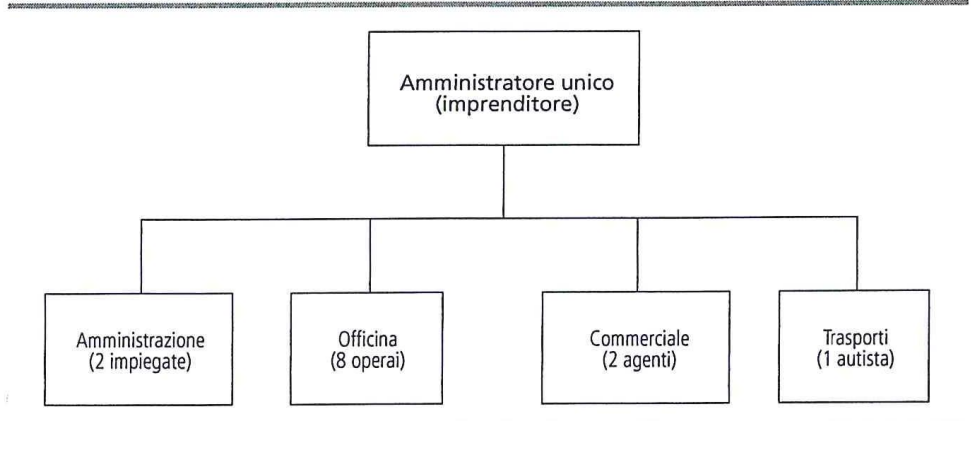
\includegraphics[width=1\textwidth]{images/elementare.png}
    \caption{Struttura Elementare}
\end{figure}
\FloatBarrier
\begin{figure}[!htb]
    \centering
    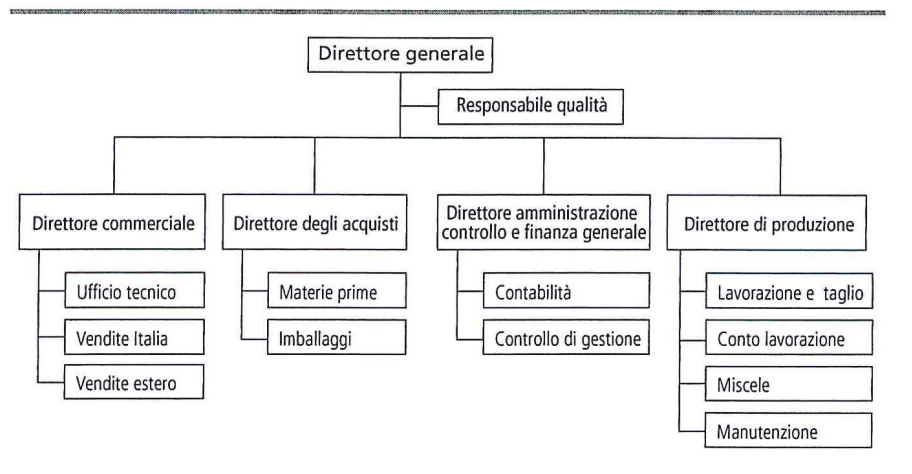
\includegraphics[width=1\textwidth]{images/funzionale.png}
    \caption{Struttura Funzionale}
\end{figure}
\FloatBarrier
\begin{figure}[!htb]
    \centering
    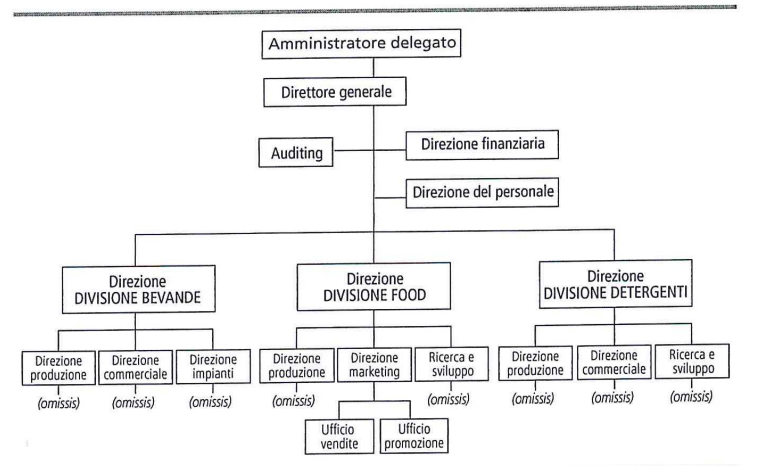
\includegraphics[width=1\textwidth]{images/multidivisionale.png}
    \caption{Struttura Multidivisionale}
\end{figure}
\FloatBarrier
\begin{figure}[!htb]
    \centering
    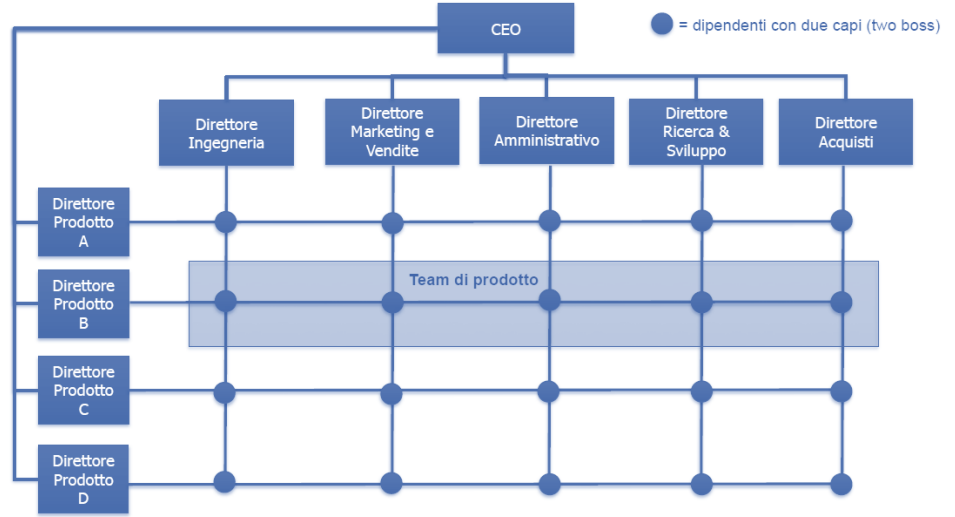
\includegraphics[width=1\textwidth]{images/matriciale.png}
    \caption{Struttura Matriciale}
\end{figure}
\FloatBarrier
\section{I Sistemi Operativi}
\begin{itemize}
    \item \textbf{Sistemi di pianificazione, gestione, controllo}
    \item \textbf{Sistemi di gestione del personale}
    \item \textbf{Sistema informativo aziendale}
\end{itemize}
\newpage
\section{Classificare le imprese}
\subsection{Secondo la produzione}
\begin{itemize}
    \item Primario
    \item Secondario
    \item Terziario (avanzato)
          \begin{itemize}
              \item Natura \textbf{immateriale} dell'output
              \item Necessaria una \textbf{contestualità} della produzione o del consumo dell'output
              \item \textbf{Personale fondamentale}
          \end{itemize}
\end{itemize}
\subsection{Secondo la natura del soggetto economico}
\paragraph{Soggetto Economico} La \textit{persona} o \textit{insieme di persone} che detiene il \textbf{potere formale di governo dell'impresa}
\begin{itemize}
    \item \textbf{Pubbliche}: proprietà di un \textit{soggetto giuridico pubblico}
    \item \textbf{Private}: proprietà di un \textit{soggetto giuridico privato} o di un loro \textit{gruppo}
    \item \textbf{Miste (o a capitale misto)}: imprese che prevedono un \textit{capitale di rischio} conferito in parte da \textit{soggetti pubblici} e in parte da \textit{soggetti privati} in varia proporzione a seconda della genesi e dello scopo della partnership
\end{itemize}
\subsubsection{Imprese quotate in borsa}
Imprese (tra le quali anche miste) i cui azionisti hanno deciso di accedere ai mercati borsistici. Una parte più o meno ampia del capitale di rischio è soggetta a una \textbf{compravendita} sul mercato.
\begin{itemize}
    \item \textbf{Soggetto economico frammentato}
    \item \textbf{Facilmente contendibile da soci di minoranza organizzati}
    \item \textbf{Induce a comportamenti a breve termine per aumentare il valore azionario}
    \item \textbf{Obblighi sulla gestione} (es. resoconto trimestrale) per tutelare il pubblico risparmio
\end{itemize}
\subsection{Secondo la forma giuridica}
\begin{itemize}
    \item \textbf{Impresa individuale}: il singolo imprenditore è l'unico responsabile della gestione anche se può avvalersi di collaboratori e/o dipendenti
    \item \textbf{Impresa collettiva o società}: L'impresa nasce dall'\textbf{accordo tra due o più persone} intenzionate a svolgere insieme l'attività. I membri del \textit{soggetto economico} sono detti \textbf{soci}. Essi sono tenuti a dare un contributo all'impresa attraverso il conferimento di beni/servizi con modalità diverse definite dallo \textit{statuto della società} e dalle \textit{norme del codice civile}
          \begin{itemize}
              \item \textbf{Società di persone}: soggetto \textit{giuridico} rappresentato dall'insieme di \textit{tutte} le \textbf{persone socie} e a queste fanno capo \textit{tutti} i \textbf{diritti} e i \textbf{doveri} che scaturiscono dall'attività
              \item \textbf{Società cooperativa}: società con scopo \textbf{mutualistico}, ovvero non di realizzare utili da cedere ai soci, ma di cedere ai beni/servizi stessi per diminuirne il prezzo
              \item \textbf{Società di capitale}:
                    \begin{itemize}
                        \item \textbf{Società per azioni}: esercitano l'attività di impresa usando come \textit{mezzi propri} il \textit{patrimonio conferito} ai soci tramite le \textbf{azioni}
                        \item \textbf{Società a responsabilità limitata}: ideale per imprenditori che vogliono salvaguardare il proprio capitale
                    \end{itemize}
          \end{itemize}
\end{itemize}
\begin{figure}[!htb]
    \centering
    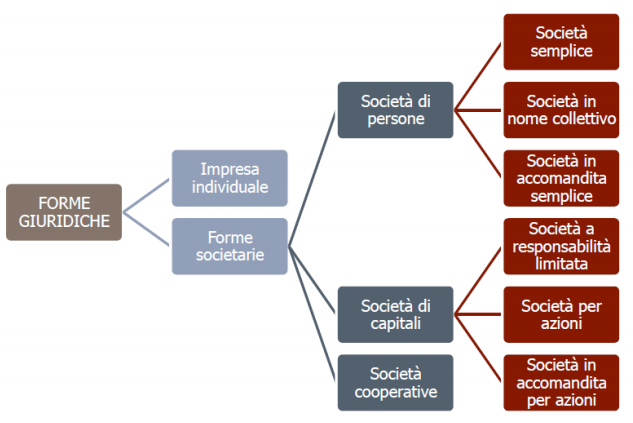
\includegraphics[width=1\textwidth]{images/giuridica.png}
    \caption{Classificazione Giuridica}
\end{figure}
\FloatBarrier
\subsection{Estensione dell'attività}
Lo sviluppo dell'impresa può avvenire lungo 3 direzioni:
\begin{itemize}
    \item \textbf{Estensione verticale} a cui corrisponderà un'\textbf{Integrazione verticale}
    \item \textbf{Estensione orizzontale} a cui corrisponderà una \textbf{Diversificazione}
    \item \textbf{Estensione geografica} a cui corrisponderà una \textbf{Internazionalizzazione}
          \begin{itemize}
              \item \textbf{Vantaggi}
                    \begin{itemize}
                        \item Supply Chain estese
                        \item Multisourcing
                        \item Minori costi del lavoro
                        \item Minore tutela dei diritti
                        \item Minore tutela dell'ambiente
                        \item Meno regole
                        \item Minore fiscalità
                    \end{itemize}
              \item \textbf{Svantaggi}
                    \begin{itemize}
                        \item Rischio disruption
                        \item Motivi naturali
                        \item Motivi politici
                        \item Motivi sanitari
                    \end{itemize}
          \end{itemize}
\end{itemize}
\paragraph{Vulnerabilità e Resilience} Capacità di resistere a eventi avversi
\newpage
\section{Contabilità e Bilancio}
\subsection{Classificazione dei conti: Reddituali vs. Patrimoniali}
\paragraph{Conti reddituali (annuali)} Vi confluiscono:
\begin{itemize}
    \item \textbf{Costi}: componenti negativi di reddito. Esprimono il valore dei fattori produttivi acquisiti per lo svolgimento della gestione.
    \item \textbf{Ricavi}: componenti positivi di reddito. Corrispondono al valore dei beni/servizi ceduti
\end{itemize}
La contrapposizione tra costi e ricavi consente di misurare il \textbf{risultato economico}.
\paragraph{Conti patrimoniali (grandezze cumulate o di fondo)} Vi vengono inseriti valori che misurano:
\begin{itemize}
    \item La consistenza del \textbf{patrimonio} aziendale
          \begin{itemize}
              \item Disponibiltà liquide
              \item Crediti in particolare finanziari
              \item Beni a utilità pluriennale: Immobilizzazioni materiali e Immateriali
          \end{itemize}
    \item La consistenza delle \textbf{fonti} di finanziamento
          \begin{itemize}
              \item Debiti in particolare finanziari
              \item Capitale sociale e riserve
          \end{itemize}
\end{itemize}
\subsection{Oggetto della registrazione}
Si registrano operazioni di \textbf{scambio monetario}: si registra solo il \textbf{valore} dei beni nella \textbf{moneta} (di conto) del paese sede dell'azienda
\paragraph{Scambio monetario} L'azienda acquista (o vende) \textbf{beni/servizi}, dando o ricevendo in cambio
\begin{itemize}
    \item \textbf{Moneta} o
    \item \textbf{Credito} (rispetto ai clienti)/\textbf{Debito} (rispetto ai fornitori)
\end{itemize}
Il \textbf{credito/debito} è una forma temporaneamente \textbf{sostitutiva} della moneta che \textit{viene registrato nel bilancio precisando la ragione della posta}. Consente atti di scambio a regolamento differito.
\subsection{Flussi di segno opposto}
\begin{figure}[!htb]
    \centering
    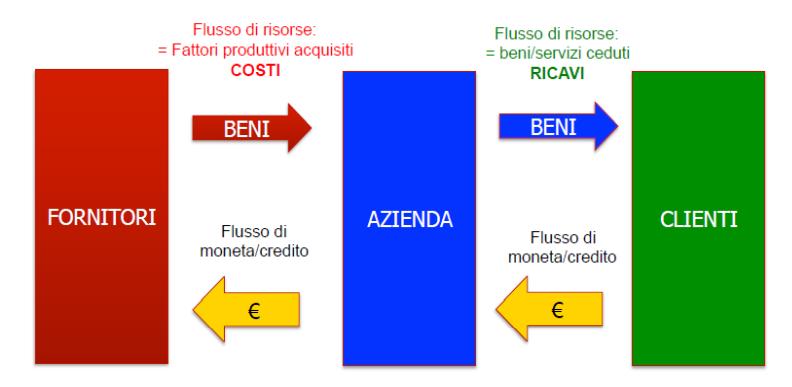
\includegraphics[width=1\textwidth]{images/flussi.png}
    \caption{Flussi di segno opposto}
\end{figure}
\FloatBarrier
\subsection{Quando si registrano i valori} I valori si raccolgono nel momento della \textbf{registrazione della fattura}
\paragraph{Partita doppia}
\begin{itemize}
    \item Il metodo di funzionamento della contabilità generale è definito partita doppia
    \item Ogni operazione origina contemporaneamente \textbf{due annotazioni} per importi \textbf{complessivamente uguali}
          \begin{itemize}
              \item In due conti distinti, e
              \item In opposte sezioni ("dare" e "avere")
          \end{itemize}
\end{itemize}
$$Dare_{TOT} = Avere_{TOT}$$

\paragraph{In Sintesi}
Durante la gestione aziendale la \textbf{contabilità generale} accoglie un flusso costante di \textbf{registrazioni} riguardanti \textbf{valori} generati da operazioni di scambio con soggetti esterni all’impresa movimentando i \textbf{conti} patrimoniali e reddituali con l'inserimento di \textbf{valori certi e incontrovertibili}, detti \textbf{quantità economiche}

\subsection{Bilancio d'esercizio: Finalità e Struttura}
Per le finalità di conoscenza interne ed esterne occorre "interrompere" la gestione per misurare i risultati in un certo arco di tempo.
Si redige quindi il \textbf{bilancio d'esercizio} per un \textbf{periodo amministrativo} (di durata annuale tipicamente)

\subsection{Bilancio: Sintesi}
\textbf{2 tavole}
\begin{itemize}
    \item Stato Patrimoniale
    \item Conto Economico
    \item Nota Integrativa
    \item Relazione sulla Gestione
    \item Rendiconto Finanziario
\end{itemize}
\paragraph{Stato Patrimoniale} Esprime la consistenza e la composizione degli investimenti e delle fonti di finanziamento dell'azienda alla data di chiusura dell'esercizio. Composto da \textbf{attivo} e \textbf{passivo}, di \textbf{pari importo}.
\subparagraph{Attivo (IMPIEGHI)}
\begin{itemize}
    \item Attività Immobilizzate: Sono risorse impiegate per l'acquisto di beni ad utilità pluriennale
    \item Attività Correnti: Sono risorse di diversa provenienza destinate a "trasformarsi in liquidità" entro l'esercizio successivo  Tra queste anche il capitale circolante
\end{itemize}
\subparagraph{Passivo (FONTI DI FINANZIAMENTO)}
\begin{itemize}
    \item Passività a Medio/Lungo termine: Sono risorse finanziarie fornite da terzi alla società e destinate ad una restituzione oltre l'esercizio successivo
    \item Passività Correnti: Sono risorse finanziarie fornite da terzi alla società e destinate ad una restituzione nell'esercizio successivo
    \item Patrimonio Netto: Rappresenta il valore delle risorse finanziarie fornite dagli azionisti in vari momenti della vita della società (alla costituzione e in momenti successivi sotto forma di capitale sociale e in itinere per utili non distribuiti). Si tratta di un finanziamento permanente
          \begin{itemize}
              \item Da parte dei soci
              \item Da parte dell'imprenditore
              \item Attraverso il reinvestimento nell'azienda stessa di utili
          \end{itemize}
\end{itemize}
\paragraph{Conto Economico} Il conto economico contiene i ricavi e i costi dell'esercizio che riassumono gli accadimenti che hanno caratterizzato la combinazione produttiva nell'arco dei 12 mesi. Il conto economico permette di determinare analiticamente le modalità di formazione del \textbf{risultato di periodo}.
\subparagraph{REDDITO D'ESERCIZIO $\neq$ ENTRATA MONETARIA}
Possibile, per esempio, che un’azienda rilevi un utile di esercizio, ma sia in situazione “critica” per quanto riguarda le disponibilità liquide.
\paragraph{Nota Integrativa} La nota integrativa ha una funzione descrittiva ed esplicativa: commenta i singoli valori, ne giustifica le variazioni rispetto all’esercizio precedente, ne fornisce dettagli e scomposizioni.
\paragraph{Relazione sulla Gestione} Fornisce indicazioni su elementi rilevanti per l’apprezzamento della situazione aziendale quali, per esempio: condizioni di ambiente economico, andamento dei mercati di riferimento, attività di ricerca e sviluppo realizzate.
\subsection{Redazione del Bilancio}
La redazione del bilancio deve essere svolta nel rispetto del principio della \textbf{competenza economica}
\begin{itemize}
    \item Componenti Positive e Componenti Negative \textbf{correlate}
    \item Componenti Positive e Componenti Negative \textbf{imputate a quel periodo amministrativo}
    \item I ricavi sono di competenza se generati durante il periodo amministrativo
    \item I costi sono di competenza se correlati ai ricavi, ovvero se i fattori produttivi cui si riferiscono hanno fornito la propria utilità durante il periodo amministrativo.
\end{itemize}
\subsection{Valori di Bilancio}
\begin{itemize}
    \item Valori \textbf{certi e incontrovertibili (quantità economiche)} generati da operazioni di scambio con soggetti esterni all’impresa; costi del personale
    \item Valori \textbf{stimati}, cioè stime di quantità economiche il cui valore sarà definito in un tempo futuro; essi sono suscettibili di una successiva verifica; fonti di incertezza, prezzo delle materie prime, previsione delle vendite
    \item Valori \textbf{congetturati} che derivano dalla necessità di ripartire i valori relativi a processi che interessano due o più esercizi al fine di imputarli al risultato dei diversi periodi. Le congetture non sono suscettibili di una verifica ex-post, ma consentono solo la formulazione di un giudizio di carattere generale sul loro grado di congruità. \textit{Valorizzazione delle immobilizzazioni immateriali}.
\end{itemize}
\textbf{La valutazione delle ultime due categorie di valori è inevitabilmente discrezionale}
\subsection{Ammortamenti}
Il processo di ammortamento effettua la ripartizione del valore di un’immobilizzazione (costo comune a più esercizi) tra gli esercizi della sua vita utile economica.
\begin{itemize}
    \item La quota di ammortamento annua di ciascuna categoria di immobilizzazioni viene inserita tra i costi del conto economico, e contemporaneamente, contribuisce al formarsi di un fondo ammortamento, posto a rettifica del valore del bene cui si riferisce nello stato patrimoniale.
    \item Il valore contabile dell’immobilizzazione è progressivamente ridotto da questo processo: in bilancio (attivo dello stato patrimoniale) compare il valore contabile del bene al netto dell’ammortamento cumulato.
\end{itemize}
\subsection{Analisi di Bilancio}
Confronti tra voci o gruppi di voci sia di Stato Patrimoniale sia di Conto Economico di uno stesso bilancio, che danno origine a indici (calcolati in forma di rapporti) o a margini (calcolati in forma differenziale). Svolta da
\begin{itemize}
    \item Gruppo Dirigente: Pianificare, organizzare e controllare l’attività futura dell’impresa
    \item Finanziatori attuali e potenziali: Valutano la capacità di credito dell’impresa, ossia il grado di affidabilità del debitore (attuale o potenziale)
    \item Soci attuali e potenziali: Valutano la capacità di reddito della società perché sulla base della redditività della gestione si basa la "remunerabilità" del capitale investito
\end{itemize}
\paragraph{Indici di Bilancio}
\begin{itemize}
    \item Struttura Finanziaria
    \item Liquidità
    \item Rotazione
    \item Redditività
\end{itemize}
\section{Aziende, Famiglie, Mercati}
\subsection{Efficienza dei Mercati}
La funzione principale dei mercati è l’allocazione efficiente delle risorse tra le varie attività produttive. Ruolo del pubblico decisivo. Tempo e Rischio sono correlati, presenza di modelli condivisi per il time-value of money
\subsection{Famiglie/Individui}
Acquistano azioni e debito sia sovrano (titoli emessi da stati) sia corporate (obbligazioni).
\subsection{Aziende}
Chiedono soldi al mercato e vendono azioni e obbligazioni. Diagramma cash flow con incertezza. Esistono comunque rischi legati alla solidità dell’azienda.
\subsection{Cash-Flow}
Flusso di cassa (Studiare diagramma)
\subsection{Crisi 2008 USA}
\paragraph{Crisi dei subprime}
Il prezzo delle case era nel frattempo aumentato moltissimo "drogato" dai mutui facili sinchè
nel 2006 inizia a scendere. Nello stesso periodo la banca centrale USA alza i tassi temendo
l’inflazione. Tutto questo ha reso negativo il valore di molte case i cui proprietari hanno smesso di pagare il mutuo perdendo la casa che è stata ripresa dalla banca per essere messa sul mercato contribuendo ad un ulteriore declino dei prezzi. La spirale distruttiva si interrompe per l’intervento dello Stato che salva, di fatto nazionalizzando, alcune grandi banche, ed avvia in USA e UK interventi di “quantitative easing”. Acquisto di debito pubblico dalle banche per ridare liquidità al sistema delle imprese.
\paragraph{Fattore di Sconto} Valutazione di obbligazioni future come un equivalente al calcolo del valore attuale
$$FdS_1={1\over(1+r)}$$
\paragraph{VAN (Valore Attualizzato Netto)} Funzione decrescente di $r$
\paragraph{Future Value di Sequenze di Flusso di Cassa}
$$FV=x_0(1+r)^n+x_1(q+r)^{n-1}+x_2(1+r)^{n-2}+\dots+x_n$$
\paragraph{Relazione tra VA e VF}
$$FV=x_0(1+r)^n+x_1(q+r)^{n-1}+x_2(1+r)^{n-2}+\dots+x_n$$
$$PV=x_0+{x_1\over(1+r)^1}+{x_2\over(1+r)^2}+\dots+{x_n\over(1+r)^n}$$
$$(1+r)^nPV=FV \Longleftrightarrow {PV = {FV\over{(1+r)^n}}}$$
Per approvare un progetto deve avere NPV positivo
\paragraph{Payback} Rappresenta il tempo necessario per recuperare l'investimento iniziale $CF_0$. Usato per valutare progetti semplici e brevi
\paragraph{ARR (Average Rate Return)} Stima della redditività che mette in relazione l'investimento iniziale $CF_0$ con la media dei cash flow attesi. Interpretabile come il tasso medio di ritorno atteso dal progetto.
\paragraph{IRR} Vedere wikipedia
\subsection{Short Position}
\begin{enumerate}
    \item Prestito di shares a prezzi bassi da un broker
    \item Vendita sul mercato al market price
    \item Quando il market price scende, ricomprarle
    \item Ritornare al broker le shares
\end{enumerate}
\subsection{Gli strumenti derivati (Contratti a Termine)}
Valore dipendente da un asset sottostante. Consentono di scambiare beni disponibili in futuro ad un prezzo che viene determinato al momento della stipulazione del contratto.
\begin{itemize}
    \item \textbf{Futures}: il contratto configura un obbligo (scadenza) per entrambe le parti. Il contratto ha costo zero. Pagamento giornaliero del credito/debito.
    \item \textbf{Opzioni}: il contratto ha un costo. La parte che vende il contratto opzione riceve il prezzo e si obbliga all'esecuzione del contratto, la parte che compra non ha obblighi ma solo l'opzione di esercitare il contratto se risulta conveniente cioè il payoff è maggiore del prezzo pagato.
\end{itemize}
\paragraph{Caratteristiche}
\begin{itemize}
    \item Danno vita ad un mercato che esprime prezzi che incorporano in modo esplicito le aspettative degli operatori economici sui prezzi futuri
    \item Ci sono prevalentemente due posizioni per quanto riguarda i contratti future:
          \begin{itemize}
              \item  La parte che assume una posizione lunga (long) è obbligato ad acquistare dall’altra parte l’ammontare di «beni» stabilito nel contratto al prezzo in esso stabilito ad una certa data.
              \item La posizione corta (short) è quella contraria, è obbligata a consegnare l’ammontare di beni stabilito al prezzo e data stabiliti
              \item La prima esigenza che dà origine a questo tipo di contratto è quella di bloccare il prezzo futuro, garantirsi, quindi, contro il rischio di eccessive variazioni. Per questa ragione il future su materie prime è utilizzato da aziende per la proprie materie prime.
          \end{itemize}
\end{itemize}
\paragraph{Opzioni}
Le opzioni sono strumenti finanziari che danno al compratore il diritto, ma non il dovere, di
comprare, nel caso di option call, o di vendere, nel caso di option put, una quantità
determinata di un’attività finanziaria o reale sottostante ad un prezzo determinato, ad una data
specificata oppure entro una data specificata.
\\
Il premio che l’acquirente dell’opzione paga al venditore rappresenta il valore di tale diritto.
\\
Quando l’acquisto di un’opzione conferisce il diritto di acquistare l’attività sottostante, l’opzione è definita di tipo \textit{call}, mentre quando conferisce il diritto di vendere l’attività sottostante è di tipo \textit{put}.
\\
L’opzione è definita un contratto \textbf{asimmetrico} in quanto implica rischi e potenziali guadagni diversi per l’acquirente e il venditore. L’acquirente ha un costo certo, che è dato dal premio pagato anticipatamente e guadagni potenzialmente illimitati o al massimo pari al prezzo strike meno il premio pagato. Mentre il venditore ha un guadagni certo costituito dal premio incassato ma ha perdite potenzialmente illimitate.
\\
Gli elementi fondamentali che compongono un contratto di opzione sono i seguenti:
\begin{itemize}
    \item \textbf{Premio}: è il prezzo che viene pagato all’acquisto dell’opzione e che non è restituibile all’investitore, sia che l’opzione venga esercitata o meno.
    \item \textbf{Prezzo di esercizio o prezzo di base (strike price)}: è il prezzo a cui l’investitore, esercitando il diritto incorporato nell’opzione, compra o vende il sottostante.
    \item \textbf{Sottostante}: gli indici o le singole azioni su cui vengono stipulate le opzioni.
    \item \textbf{Scadenza}: può essere di tipo europeo (l’acquirente può esercitare l’opzione solo alla scadenza del contratto) o americano (l’acquirente può esercitare l’opzione in ogni momento, prima della scadenza).
\end{itemize}
\newpage
\section{Microeconomia}
Ramo dell’economia che si occupa del comportamento di singoli agenti economici - consumatori, imprese, lavoratori e investitori - e dei mercati da essi costituiti.
\begin{itemize}
    \item \textbf{Consumatori}: I consumatori percepiscono redditi limitati, che possono spendere in un’ampia gamma di beni e servizi, oppure risparmiare per il futuro.
    \item \textbf{Imprese}: Anche le imprese devono affrontare limitazioni relative ai tipi di beni che possono produrre e alle risorse disponibili per produrli. (CAPITALE, LAVORO, Tecnologia)
    \item \textbf{Lavoratori}: Anche i lavoratori devono affrontare vincoli e trade-off. In primo luogo, le persone devono decidere se e quando entrare a far parte della forza lavoro. In secondo luogo, i lavoratori devono affrontare un trade-off nella scelta del posto di lavoro (interesse del lavoro vs. distanza). Infine, I lavoratori devono talvolta decidere quante ore settimanali lavorare, ovvero devono affrontare un trade-off tra lavoro e tempo libero.Scelta del telelavoro.Le modalità di lavoro stavano già cambiando, il COVID ha accelerato questo processo.
\end{itemize}
\section{Macroeconomia}
Ramo dell’economia che si occupa di grandezze economiche aggregate, come il livello e il tasso di crescita del prodotto interno lordo, dei tassi di interesse, della disoccupazione e dell’inflazione. Campo di intervento soprattutto dello stato nazionale e delle istituzioni europee.
\subsection{Prezzi e Mercati}
\begin{itemize}
    \item \textbf{Economia Pianificata}: I prezzi sono stabiliti dal governo. Le imprese sono tipicamente controllate dal governo e indirizzate a produrre una gamma ristretta di prodotti
    \item\textbf{Economia di Mercato}: I prezzi sono determinati dalle interazioni tra consumatori, lavoratori e imprese. Queste interazioni hanno luogo nei mercati – insiemi di acquirenti e venditori che, esprimendo domanda e offerta, determinano il prezzo di un bene.
\end{itemize}
\subsection{Che cos'è un mercato}
Insieme degli acquirenti e dei venditori che, attraverso le loro interazioni effettive o potenziali, determinano il prezzo di un prodotto o di un gruppo di prodotti. Capire o addirittura prevedere il comportamento dei soggetti attivi in un mercato , in particolar
modo dei consumatori (ma anche dei produttori) è l’obiettivo del marketing (a diversi livelli di aggregazione).
\begin{itemize}
    \item \textbf{Mercato perfettamente concorrenziale}: Mercato in cui operano molti acquirenti e venditori e in cui, quindi, nessuno di essi, singolarmente, può influenzare in modo significativo il prezzo. Esistono molti mercati con un livello di concorrenzialità tale da poter essere considerati perfettamente concorrenziali.
    \item \textbf{Mercato non concorrenziale}: Alcuni mercati (materie prime, ad esempio petrolio), comprendono molti produttori ma sono non concorrenziali in quanto le singole imprese (spesso statali) sono in grado, accordandosi tra loro, di influenzare il prezzo.Accordi (cartelli) che limitano la concorrenza sono illegali e perseguibili anche penalmente. In taluni casi sono invece ufficiali.
\end{itemize}
\newpage
\section{Domanda e Offerta}
\subsection{Curva di Offerta}
\textit{Relazione tra la quantità di un bene che i produttori sono disposti a vendere e il prezzo del bene}. Questa curva è inclinata positivamente: maggiore è il prezzo, più imprese possono e desiderano produrre e vendere. Variabile che influenza l'offerta è relativa ai \textbf{costi di produzione}, che comprendono i salari, gli interessi passivi sui capitali investiti, il costo delle materie prime e di eventuali licenze. Quando i costi di produzione diminuiscono, la produzione aumenta indipendentemente dal prezzo di mercato. L’intera curva di offerta si sposta quindi verso destra
\FloatBarrier
\begin{figure}[!htb]
    \centering
    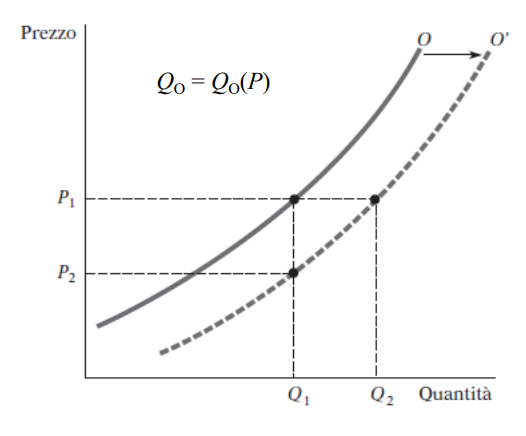
\includegraphics[width=1\textwidth]{images/offerta.png}
    \caption{Curva di Offerta}
\end{figure}
\subsection{Curva di Domanda}
\textit{Relazione tra la quantità di un bene che i consumatori sono disposti ad acquistare e il prezzo del bene}. Questa curva è inclinata negativamente: mantenendo costanti gli altri fattori, i consumatori saranno disposti ad acquistare maggiori quantità di un bene quando il
prezzo di quest’ultimo diminuisce. La quantità domandata può dipendere anche da altre variabili, come il reddito, il clima e i prezzi di altri beni. Per la maggior parte dei prodotti, la quantità domandata aumenta al diminuire del prezzo.
\FloatBarrier
\begin{figure}[!htb]
    \centering
    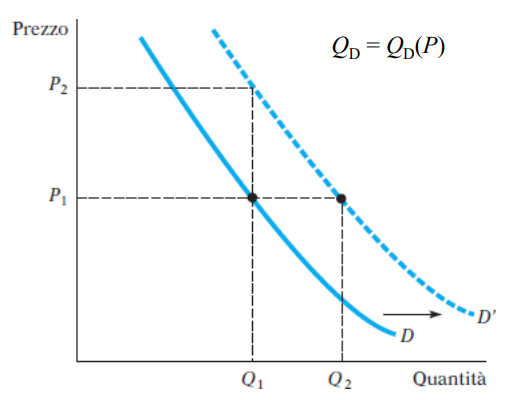
\includegraphics[width=1\textwidth]{images/domanda.png}
    \caption{Curva di Domanda}
\end{figure}
\subsection{Meccanismo di Mercato}
\begin{itemize}
    \item Il mercato è in equilibrio al prezzo $P_0$ e alla quantità $Q_0$.
    \item Al prezzo più alto $P_1$ si sviluppa un’eccedenza, che fa diminuire il prezzo.
    \item Al prezzo più basso $P_2$ si determina una scarsità, che fa aumentare il prezzo.
\end{itemize}
\FloatBarrier
\begin{figure}[!htb]
    \centering
    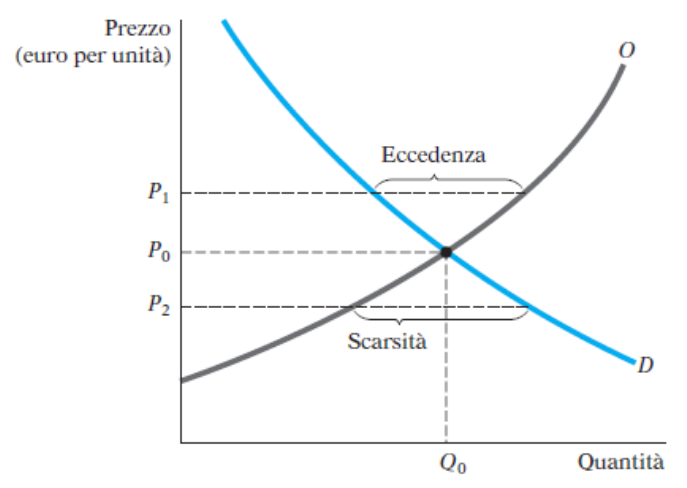
\includegraphics[width=1\textwidth]{images/mercato.png}
    \caption{Meccanismo di Mercato}
\end{figure}
\begin{itemize}
    \item \textbf{Prezzo di equilibrio} Prezzo al quale la quantità domandata e la quantità offerta si equivalgono.
    \item \textbf{Meccanismo di mercato} Nei mercati liberi, tendenza del prezzo a variare fino a quando quantità domandata e quantità offerta si equivalgono.
    \item \textbf{Eccedenza} Situazione in cui la quantità offerta supera la quantità domandata.
    \item \textbf{Scarsità} Situazione in cui la quantità domandata supera la quantità offerta.
\end{itemize}
\subsection{Elasticità della Domanda e dell'Offerta}
Variazione percentuale di una variabile prodotta dall’incremento di un punto percentuale di un’altra variabile. Non dipende solo dal suo prezzo ma anche dai redditi dei consumatori e dai prezzi di altri beni. Il "pricing" di un prodotto dipende da una valutazione quantitativa della elasticità rispetto al prezzo. Questo vale sia sul breve termini (sconti, facilitazioni) sia sul lungo termine.
\paragraph{Elasticità della domanda rispetto al prezzo} Variazione percentuale della quantità domandata di un bene prodotta da un aumento dell’1 per cento del prezzo
$$E_p={\% \Delta Q \over{\% \Delta P }}$$
\paragraph{Elasticità della domanda rispetto al reddito}
Variazione percentuale della quantità domandata prodotta da un incremento di un punto percentuale del reddito.
\paragraph{Elasticità incrociata della domanda}
Variazione percentuale della quantità domandata di un bene prodotta dall’aumento di un punto percentuale del prezzo di un altro bene
\paragraph{Elasticità dell’offerta rispetto al prezzo}
Variazione percentuale della quantità offerta prodotta da un incremento di un punto percentuale del prezzo
\subsection{Analisi Domanda-Offerta}
\begin{itemize}
    \item Valutare l’impatto degli interventi pubblici
    \item Comprendere e prevedere come le variazioni delle condizioni economiche mondiali nazionali e locali influiscono sul prezzo di mercato e sui costi di produzione
    \item Determinare gli effetti sui consumatori e sui produttori di tasse, sussidi, dazi doganali e quote alle importazioni
    \item Sanzioni politiche
\end{itemize}
\newpage
\section{Comportamento del Consumatore}
\subsection{Teoria del comportamento del consumatore}
Descrive come ogni consumatore distribuisce il proprio reddito tra differenti beni e servizi per massimizzare il proprio welfare-benessere-soddisfazione-utilità.
\begin{itemize}
    \item Preferenze del consumatore: utilità di un bene
    \item Vincoli di bilancio
    \item Scelte del consumatore
\end{itemize}
\textbf{Panieri (Basket) di mercato = Diverse scelte del consumatore}
\paragraph{Ipotesi sulle preferenze}
\begin{itemize}
    \item \textbf{Transitività}: se un consumatore preferisce il paniere A al paniere B e il paniere B al paniere C, allora preferirà A a C. La transitività è di solito considerata necessaria per la coerenza del consumatore
    \item \textbf{Di più è meglio che di meno}: Si assume che i beni siano desiderabili
\end{itemize}
\subsection{Recommender Systems}
L’ipotesi di perfetta concorrenzialità dei mercati si accompagna alla perfetta e completa informazione: questo non è raggiunto nei mercati reali anche digitali. \\
L’informazione in tutti i mercati ha un costo ed è un importante differenziatore tra i vari attori del mercato (ad esempio consumatori e produttori).
Importanza dei «recommender systems» (Netflix, Amazon, ...) che in base alle preferenze dell’utente , in base al profili utente, i ratings pregressi e le info tratte da social networks acquisite on line indicano al singolo consumatore gli item preferiti.\\
I recommender danno un’informazione ma è certamente "biased" e incompleta.
Esistono anche sistemi di aggregazione e comparazione che dovrebbero essere
indipendenti dai produttori e aiutare in modo unbiased i consumatori nella scelta.
\subsection{Curva di indifferenza}
Curva che rappresenta tutte le combinazioni di panieri che garantiscono a un consumatore lo stesso livello di soddisfazione. La scelta tra questi dipende da caratteristiche personali del consumatore riassunte nella curva di indifferenza
\FloatBarrier
\begin{figure}[!htb]
    \centering
    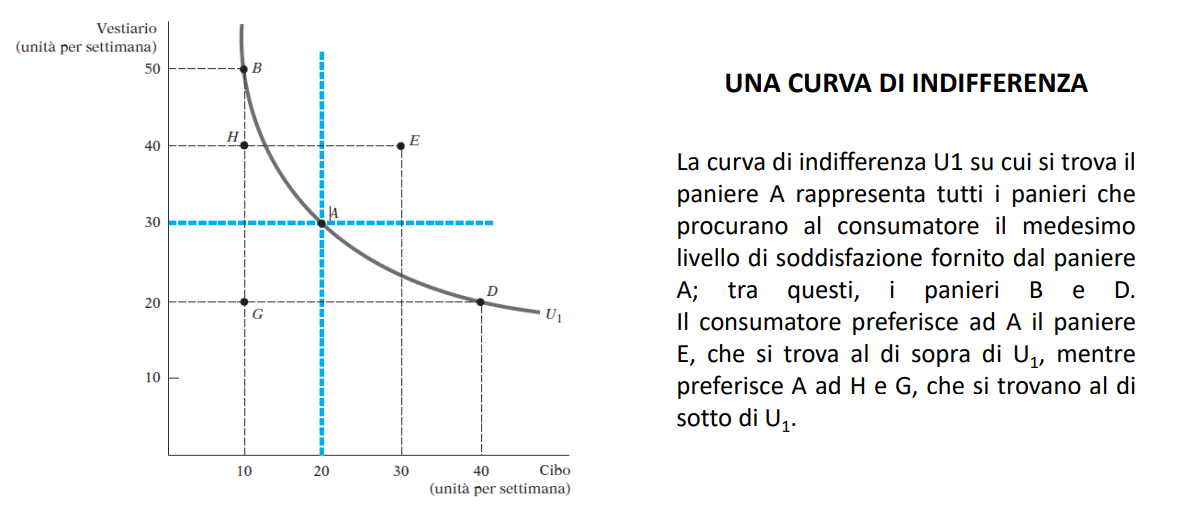
\includegraphics[width=1\textwidth]{images/curvaInd.png}
    \caption{Curva di Indifferenza}
\end{figure}
Le curve di indifferenza sono legate alla "profilazione" di un consumatore e possono rappresentare diverse situazioni ad esempio rischio e rendimento nelle decisioni di investimento.
\subsection{Funzioni di Utilità}
\paragraph{Utilità} Valore numerico che rappresenta la soddisfazione che un consumatore ricava da un determinato paniere
\paragraph{Funzione di utilità} Formula che assegna un livello di utilità ai singoli panieri.
Una funzione di utilità può essere rappresentata da una serie di curve di
indifferenza, ciascuna associata a un indicatore numerico. Questa figura mostra tre curve di indifferenza (corrispondenti ai livelli di
utilità 25, 50 e 100, rispettivamente) associate alla funzione CV
$$u(C,V)=C \times V$$
\FloatBarrier
\begin{figure}[!htb]
    \centering
    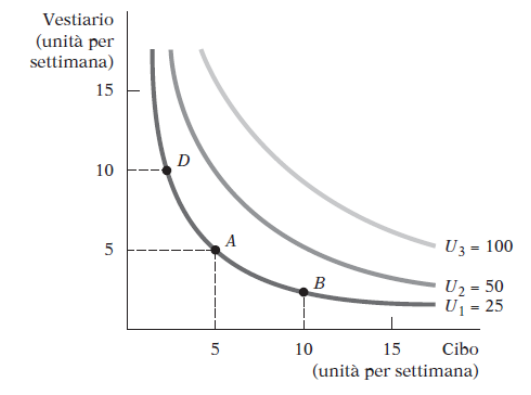
\includegraphics[width=1\textwidth]{images/fUtil.png}
    \caption{Funzione di Utilità}
\end{figure}
\subsection{Vincoli di Bilancio}
Vincoli che i consumatori affrontano a causa dei reddito limitati.
\paragraph{Retta di Bilancio}
Tutte le combinazioni di beni per le quali la somma di denaro spesa è
uguale al reddito
$$P_CC+P_VV=RD$$
La retta di bilancio descrive le combinazioni di beni che possono essere acquistate dati il reddito del consumatore e i prezzi dei beni.
\FloatBarrier
\begin{figure}[!htb]
    \centering
    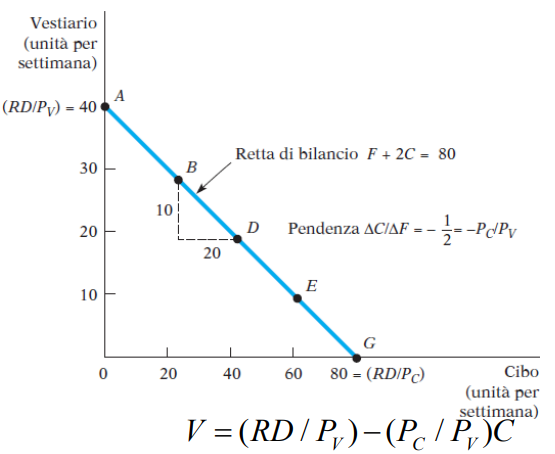
\includegraphics[width=1\textwidth]{images/rBilancio.png}
    \caption{Retta di Bilancio}
\end{figure}
\textit{Il paniere che massimizza la soddisfazione deve rispettare due
    condizioni:}
\begin{itemize}
    \item \textbf{Deve trovarsi sulla retta di bilancio}
    \item \textbf{Deve fornire al consumatore la combinazione più gradita di beni e servizi}
\end{itemize}
\subsection{Comportamento del consumatore}
\begin{itemize}
    \item Quantificare il rischio
    \item Esaminare le preferenze delle persone rispetto al rischio
    \item Come le persone possano ridurre o eliminare il rischio
    \item Analizzare come le persone scelgono quale livello di rischio accettare
\end{itemize}
\paragraph{Descrivere il rischio}
\begin{itemize}
    \item Probabilità
    \item Valore atteso: misura la tendenza centrale – il payoff o valore che ci si aspetta in media.
    \item Payoff
\end{itemize}
Consideriamo l’utilità che un consumatore ricava dal proprio reddito, o meglio dal paniere che il reddito consente di acquistare.
Misuriamo quindi i payoff in termini di utilità invece che in euro. L’utilità è una funzione monotona crescente della variabile monetaria.
\\\\
\textit{Un consumatore ha un reddito di $€15.000$, che associa ad una utilità di $13.5$, e sta prendendo in considerazione una nuova ma «rischiosa» occupazione (ad esempio un’attività di vendita con una importante componente variabile) che potrebbe raddoppiare il suo reddito portandolo a $€30.000$, oppure farlo scendere a $€10.000$. Ognuna delle due possibilità ha probabilità di $0.5$. Il livello di utilità associato a $10000$ è $10$ mentre quello associato a $30000$ è $18$. Per valutare il nuovo lavoro, il consumatore calcola il valore atteso del reddito risultante.\\
    Poiché stiamo misurando il valore in termini di utilità, dobbiamo calcolare l’utilità attesa $E(u)$ che il consumatore può conseguire:}
\paragraph{Utilità attesa} Somma delle utilità associate a tutti i possibili esiti, pesate dalle probabilità che i rispettivi esiti si verifichino.
$$E(u) = {1\over 2}u \times {10000} + {1\over 2}u \times {30000} = 0.5 \times 10 + 0.5 \times 13.5 = 14$$
\textit{\textbf{Il nuovo lavoro rischioso sarebbe preferibile a quello attuale, perché la sua utilità attesa, 14, è maggiore di quella di partenza, 13.5}}
\paragraph{Avversione al rischio} Preferenza per un reddito certo rispetto a un reddito rischioso avente lo stesso valore atteso. Le persone sono diverse per quanto riguarda la propensione al rischio.
\paragraph{Premio di rischio} Massima somma di denaro che una persona avversa al rischio è disposta a pagare per evitare il rischio.
\FloatBarrier
\begin{figure}[!htb]
    \centering
    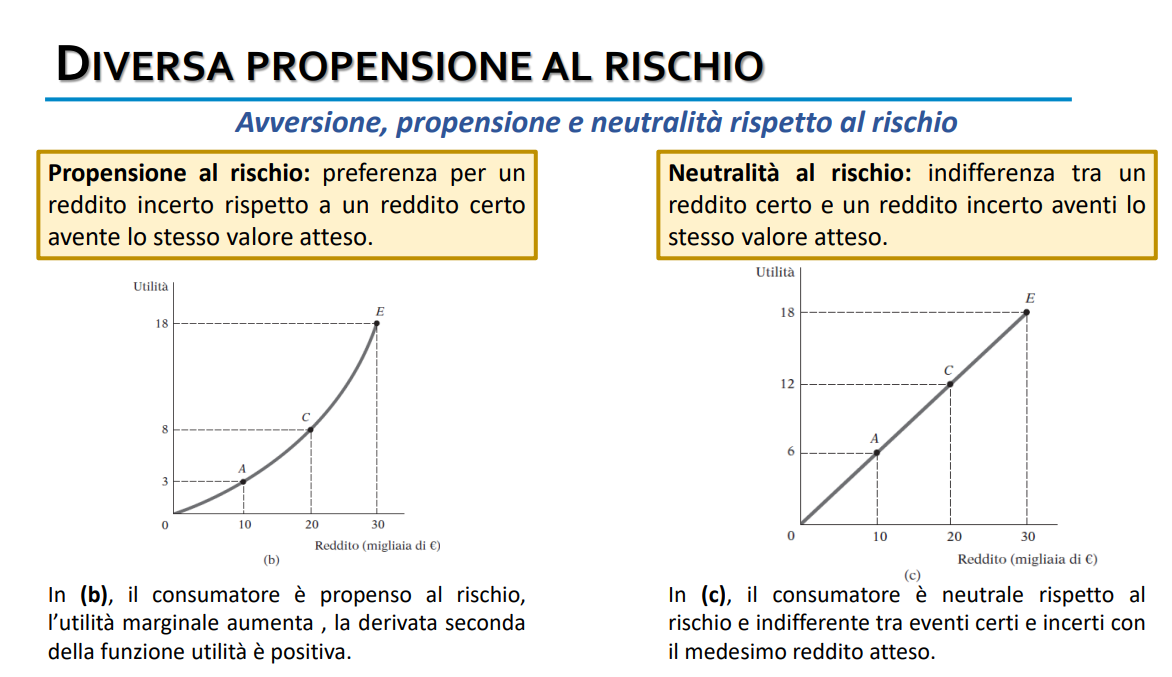
\includegraphics[width=1\textwidth]{images/propRischio.png}
    \caption{Diverse propensioni al rischio}
\end{figure}
\FloatBarrier
La propensione al rischio è correlata a "exploration/exploitation" che
è centrale in tutti i processi di apprendimento, in particolare active
learning e reinforcement learning.
\newpage
\section{Domanda Individuale e di Mercato}
\subsection{Variazione del Prezzo}
Una riduzione del prezzo del cibo, quando il reddito e il prezzo del
vestiario rimangono invariati, fa si che il consumatore scelga un
paniere differente.
\FloatBarrier
\begin{figure}[!htb]
    \centering
    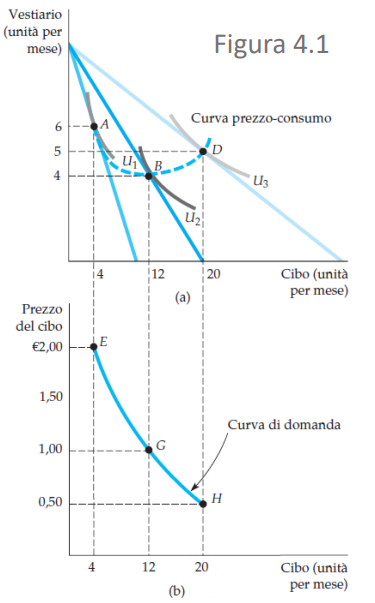
\includegraphics[width=0.5\textwidth]{images/domind.png}
\end{figure}
\FloatBarrier
In (a), i panieri che massimizzano l’utilità in corrispondenza di vari
prezzi del cibo (punto A, €2; B, €1; D, €0,50) definiscono la curva
prezzo-consumo.

In (b) è data la curva di domanda, che pone in relazione il prezzo
del cibo e la quantità domandata (i punti E, G e H corrispondono ai
punti A, B e D, rispettivamente).
\subsection{Variazione del Reddito}
Un aumento del reddito, quando i prezzi dei beni rimangono invariati, fa sì che i consumatori scelgano panieri differenti.
\FloatBarrier
\begin{figure}[!htb]
    \centering
    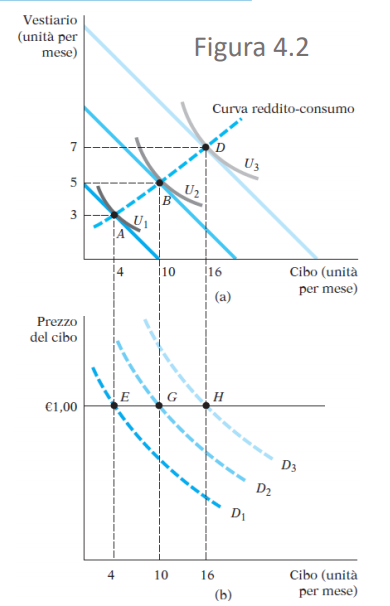
\includegraphics[width=0.5\textwidth]{images/varRed.png}
\end{figure}
\FloatBarrier

\subsection{Sostituti e Complementi}
\begin{itemize}
    \item Due beni sono \textbf{sostituti} se l’aumento del prezzo dell’uno conduce all’aumento della quantità domandata dell’altro.
    \item Due beni sono \textbf{complementi} se l’aumento del prezzo dell’uno conduce alla diminuzione della quantità domandata dell’altro.
    \item Due beni sono \textbf{indipendenti} se la variazione del prezzo dell’uno non ha effetti sulla quantità domandata dell’altro.
\end{itemize}
\subsection{Esternalità di Rete}
Situazione in cui la domanda di ciascun individuo dipende dagli acquisti
effettuati dagli altri individui.\\
Un’\textbf{esternalità di rete positiva} si ha quando la quantità di un bene domandata da un tipico consumatore (o il valore associato WTP Willingness to pay) aumenta all’aumentare della quantità acquistata dagli altri consumatori. Se invece la quantità domandata diminuisce, si ha una \textbf{esternalità di rete negativa (snob)}.
\paragraph{Effetto Traino} Esternalità di rete positiva in virtù della quale un consumatore desidera possedere un bene anche perché altri lo possiedono.
\paragraph{Sondaggi}
\subsection{Domanda di Mercato}
\paragraph{Curva di domanda di mercato} Curva che esprime la relazione tra la quantità di un bene che tutti i consumatori di un mercato acquistano e il prezzo del bene.
\newpage
\section{Marketing}
\begin{itemize}
    \item Automazione della produzione consente livelli di flessibilità e versatilità più elevati, orientamento al cliente
    \item Tecniche ICT consentono un rapporto con il cliente individuale (social media) e un avvicinamento tra le esigenze di \textbf{standardizzazione e replicazione} e quelle di \textbf{varietà e personalizzazione}
\end{itemize}
\subsection{Ruolo nell'impresa}
\begin{itemize}
    \item \textbf{Esecutivo}: bassa complessità, domanda stabile senza difficoltà di
          assorbimento, i processi decisionali dei clienti non interessano
    \item \textbf{Operativo}: poca attenzione all’analisi della domanda, attenzione alle politiche distributive e promozionali analizzandone gli effetti
    \item \textbf{Conoscitivo}: analisi delle aspettative del consumatore e del comportamento della concorrenza
    \item \textbf{Strategico}: il marketing interviene, definisce e aggiorna nella fase di formulazione di strategie di segmentazione e di definizione e posizionamento delle linee prodotti
\end{itemize}
\subsection{Market Basket Analysis}
Analisi dei dati aggregati, non è più possibile eseguire analisi di marketing su dati semplici come in passato mediante regressione e correlazione lineare.
Utilizzo di strumenti CRM (Customer Relationship Management) per profilare i singoli utenti.
\subsection{Analisi dell'ambiente}
\begin{itemize}
    \item \textbf{Macro-Ambiente}: Ambiente demografico, economico, fisico, tecnologico, politico e istituzionale, culturale e sociale
    \item \textbf{Micro-Ambiente}: Composto dall’impresa stessa, dai fornitori, dagli intermediari, dai clienti, dai concorrenti
\end{itemize}
Analisi volta a delineare le tendenze evolutive, le forze e le condizioni riconoscibili (\textbf{SWOT} \textit{Strenght-Weaknesses Opportunities and threats}) nell’ambiente che configurano un valore positivo (\textit{OPPORTUNITA’}) o negativo (\textit{MINACCE}) per delineare il GRADO DI ATTRATTIVITA’ DEL MERCATO, Che viene misurato con RIFERIMENTO A FATTORI quali: dimensione mercato, tasso annuale di crescita, margini di profitto, potere contrattuale dei fornitori, analisi di competitività
\subsection{Analisi della concorrenza}
\begin{itemize}
    \item Prevedere le strategie e decisioni future dei concorrenti
    \item Questione IPR, marchi, modelli e brevetti
    \item Prevedere le reazioni dei concorrenti alle decisioni dell’impresa
    \item Come si può influenzare il comportamento di un concorrente
    \item Le funzioni svolte dal prodotto
\end{itemize}
\subsection{Analisi della domanda}
\begin{itemize}
    \item Stima della domanda primaria (globale) e secondaria (specifica)
    \item Stima del potenziale di mercato che rappresenta il limite teorico massimo che la domanda di un prodotto può raggiungere considerando determinati ambiti spaziali e temporali
    \item calcolo della quota di mercato che esprime l’ammontare delle vendite di una impresa in percentuale sulle vendite complessive del mercato
    \item valutazione della elasticità della domanda secondaria rispetto al prezzo che segnala la sensibilità dei consumatori in termini di modificazione della quantità acquistata in risposta a variazioni di prezzo
    \item Valutazione della elasticità incrociata che esprime la sensibilità della domanda di prodotti dell’impresa rispetto alle variazioni di prezzo dei prodotti dei concorrenti
    \item Importanza di analizzare dati di vendite al dettaglio
\end{itemize}
\newpage
\section{Recommender Systems}
\subsection{Dati utilizzati}
\begin{itemize}
    \item \textbf{interazioni esplicite user-item} (esempio, il rating dato un utente ad un certo film o il comportamento di acquisti)
    \item \textbf{informazioni su user-item} (esempio, del testo associato agli item, le informazioni personali di un utente, etc.)
    \item \textbf{interazioni implicite user-item} (ad esempio, la cronologia di un utente
\end{itemize}
\subsection{Obiettivi di un Recommender System}
\begin{itemize}
    \item \textbf{Rilevanza} raccomandare prodotti che un utente ritiene più interessanti in base alle informazioni disponibili
    \item \textbf{Novità} suggerire prodotti che un utente potrebbe non aver ancora visto
    \item \textbf{Serendipitività} suggerire prodotti «inaspettati» ma che potrebbero piacere all’utente
    \item \textbf{Incremento della diversità} suggerire prodotti di diverso tipo per evitare di «annoiare» l’utente
\end{itemize}
\subsection{Ostacoli di un Recommender System}
\begin{itemize}
    \item L’evoluzione nel tempo delle raccomandazioni
    \item Personalizzare le raccomandazioni
    \item Il problema del Cold start
    \item La resistenza agli attacchi
    \item Privacy
\end{itemize}
\subsection{Formulazione di un problema di raccomandazione}
\begin{enumerate}
    \item \textbf{Prediction version of problem}: Predire l’opinione/giudizio di un utente (user) su un prodotto specifico (item)
    \item \textbf{Ranking version of problem}: Predire una lista di prodotti per un utente (non per forza in ordine di importanza) o una lista di utenti per un prodotto
\end{enumerate}
\subsection{Metodi Collaborative-Filtering}
Le entrate vuote della matrice di rating possono essere completate perché i rating osservati sono spesso altamente correlati tra gli user ed gli item
\paragraph{Metodi memory-based}
Noti anche come metodi \textbf{neighbourhood-based k-NN}. Sono basati sul predire il rating di un utente per un item utilizzando il concetto di vicino (o neighbourhood) similarity.
A seconda del tipo di vicino considerato possiamo avere:
\begin{itemize}
    \item Metodi User-based collaborative filtering
    \item Metodi Item-based collaborative filtering
\end{itemize}
\begin{itemize}
    \item \textbf{Vantaggio}: semplici da implementare , buona accuratezza, e le raccomandazioni ottenute sono spesso facili da spiegare (explainability)
    \item \textbf{Svantaggio}: non lavorano bene in presenza di matrici di rating altamente sparse
\end{itemize}
\paragraph{Metodi model-based}
L’idea base è trovare un "modello predittivo" capace di predire i rating relativi alle entrate sconosciute della matrice di rating. Tale modello viene descritto attraverso un certo numero di parametri che vanno appresi (learning) all’interno di un framework di ottimizzazione. Alcuni esempi di modelli model-based includono: decision tree, latent factor models, etc.
\begin{itemize}
    \item Svantaggio: molto onerosi dal punto di vista computazionale
    \item Vantaggio: più precisi rispetto ai metodi memory-based e possono operare anche con matrici di rating molto sparse
\end{itemize}

\subsection{Metodi Content-Based}
I metodi di raccomandazione che usano le informazioni relative agli user ed agli item prendono il nome di content-based. Non hanno bisogno di dati relativi a passate attività come i CF, ma su dati di profilo e metadati di oggetti correlati. Visto che non prevedono community sono meno potenti dei CF.
\FloatBarrier
\begin{figure}[!htb]
    \centering
    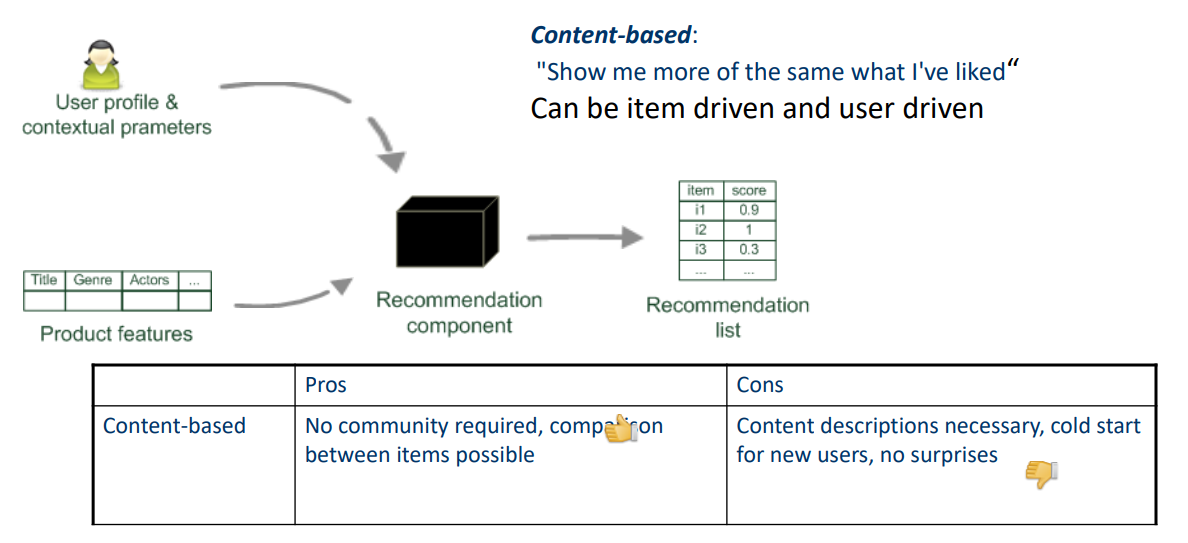
\includegraphics[width=1\textwidth]{images/CB.png}
\end{figure}
\FloatBarrier
\begin{figure}[!htb]
    \centering
    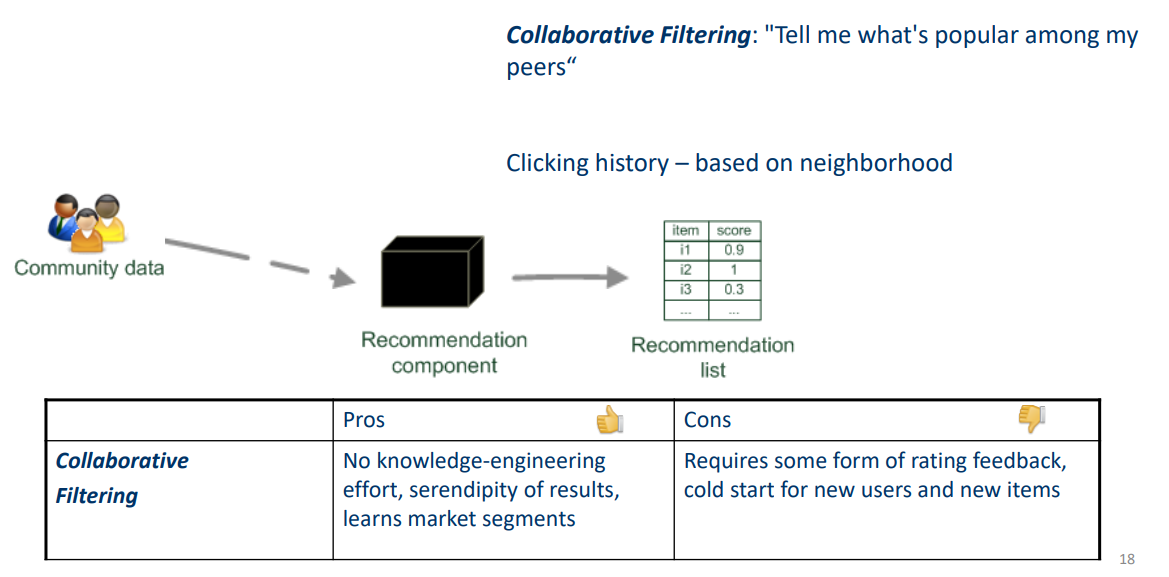
\includegraphics[width=1\textwidth]{images/CF.png}
\end{figure}
\FloatBarrier
\subsection{Rating}
I rating possono essere:
\begin{itemize}
    \item a valori continui (anche se raro)
    \item a valori interi in uno specifico intervallo (ad esempio una scala formata da 5 rating, 1-5)
    \item a valori categorici (fortemente d’accordo, d’accordo, in disaccordo, fortemente in disaccordo, neutro)
    \item a valori binari (0/1, -1/+1,dislike/like)
    \item a valori unari (1 se mi piace come in Facebook)
\end{itemize}
Le matrici di rating potrebbero non rappresentare del tutto le informazioni relative ad uno user (spesso si tende a valutare solo i film che ci piacciono). Per questo è possibile far ricorso anche a rating di tipo implicito (un film è stato visto del tutto o ci si è interrotti prima, non vengono guardati film suggeriti dal sistema, etc.)
\subsection{Cosine Similarity}
La cosine similarity rappresenta una misura di somiglianza tra 2 vettori.
Geometricamente corrisponde al coseno dell’angolo tra i due vettori. Nel caso in cui le componenti dei vettori siano non-negative (come nel caso
dei ratings), la cosine similarity può variare tra 0 (completa diversità) a +1 (massima somiglianza). È invariante rispetto alle dilatazioni. La cosine similarity può essere definite anche nel caso in cui non siano note alcune componenti dei due vettori: per farlo si considera l’insieme $I_{ab}$ come l’insieme degli indici delle componenti note sia di $a$ che di $b$, e si definisce la cosine similarity come la somma dei prodotti scalari diviso la somma dei prodotti tra i moduli
\subsection{Dati per valutare un Recommender System}
\begin{itemize}
    \item \textbf{Metodi offline}: si misura le performance di un algoritmo di raccomandazione su dei dati offline storici. Esempio: si è predetto correttamente il rating relativo ad una coppia user-item di un dataset conosciuto?
    \item \textbf{Casi studio}: si misura la reazione su un gruppo di utenti “reclutati” a cui si chiede di interagire con il sistema di raccomandazione
    \item \textbf{Metodi online}: si misura la reazione su un gruppo di utenti “veri” che interagiscono con il Sistema di raccomandazione. Esempio: un utente clicca o meno su una notizia raccomandata?
\end{itemize}
Un Recommender System può essere valutato in base a diversi criteri, tra cui:
\paragraph{Accuracy}: quanto è capace un RS di predire il rating di un utente su un item specifico? o di predire correttamente  una lista di item per uno specifico user?
\\
L’accuratezza degli algoritmi di raccomandazione può essere misurata in termini di:
\begin{itemize}
    \item \textbf{Predizione del rating}: un RS riesce a predire correttamente il rating di un utente per uno specifico item?
    \item \textbf{Predizione del ranking}: un RS riesce a predire correttamente il ranking di una lista di item per uno specifico user?
\end{itemize}
Una misura di accuratezza potrebbe essere la media delle differenze in modulo tra la previsione basata sul training e le osservazioni presenti nel test set
\newpage
\section{Parziale}
\subsection{Quali sono i documenti principali del bilancio annuale di un'azienda e le principali voci relative?}
\paragraph{Stato Patrimoniale} Esprime la \textbf{consistenza} e la \textbf{composizione} degli \textbf{investimenti} e delle \textbf{fonti di finanziamento} dell'azienda alla data di chiusura dell'esercizio. Composto da \textbf{attivo} e \textbf{passivo}, di \textbf{pari importo}.
\subparagraph{Attivo (IMPIEGHI)}
\begin{itemize}
    \item \textit{Attività Immobilizzate}: Risorse impiegate per l'acquisto di beni ad utilità pluriennale
    \item \textit{Attività Correnti}: Risorse di diversa provenienza destinate a trasformarsi in liquidità entro l'esrcizio successivo
\end{itemize}
\subparagraph{Passivo (FONTI DI FINANZIAMENTO)}
\begin{itemize}
    \item \textit{Passività a Medio/Lungo termine}: Risorse finanziarie fornite da terzi alla società e destinate ad una restituzione \textbf{oltre l'esercizio successivo}
    \item \textit{Passività Correnti}: Risorse finanziarie fornite da terzi alla società e destinate ad una restituzione \textbf{nell'esercizio successivo}
    \item \textit{Patrimonio Netto}: Rappresenta il \textbf{valore delle risorse finanziarie} fornite dagli azionisti in vari momenti della vita della società
\end{itemize}

\paragraph{Conto Economico} Contiene i \textbf{ricavi} e i \textbf{costi} dell'esercizio che riassumono gli accadimenti che hanno caratterizzato la combinazione produttiva nell'arco dei 12 mesi.

\paragraph{Nota Integrativa} \textbf{Funzione descrittiva} ed \textbf{esplicativa}: commenta i singoli valori, ne giustifica le variazioni rispetto all'esercizio precedente, ne fornisce dettagli e scomposizioni.

\paragraph{Relazione sulla Gestione} Fornisce indicazioni su elementi rilevanti per l'\textbf{apprezzamento della situazione aziendale}, ad esempio \textit{condizioni di ambiente economico, andamento dei mercati di riferimento, attività di ricerca e sviluppo realizzate}
\newpage
\subsection{Cosa si intende per Open/Closed Innovation}
L'impresa può un \textbf{sistema aperto o chiuso}.
L’impresa nel proprio ambiente di riferimento (naturale, tecnologico, sociale, istituzionale) interagisce, scambia, continuamente risorse ed energia con gli altri attori secondo un modello di \textbf{input-output}
\begin{itemize}
    \item \textit{Input}: L’organizzazione \textbf{importa} dall’ambiente esterno fattori di produzione
    \item \textit{Output}: Li \textbf{trasforma} e li \textbf{restituisce} all’esterno in forma di prodotti/servizi
\end{itemize}
\subparagraph{Aperto}
\begin{itemize}
    \item Progetti lanciati sia da basi tecnologiche/scientifiche interne che esterne
    \item Nuove tecnologie possono entrare nel flusso in diversi momenti del processo
    \item Nuove tecnologie possono andare sul mercato in tanti modi differenti (es. canali di marketing aziendali interni)
\end{itemize}
\FloatBarrier
\begin{figure}[!htb]
    \centering
    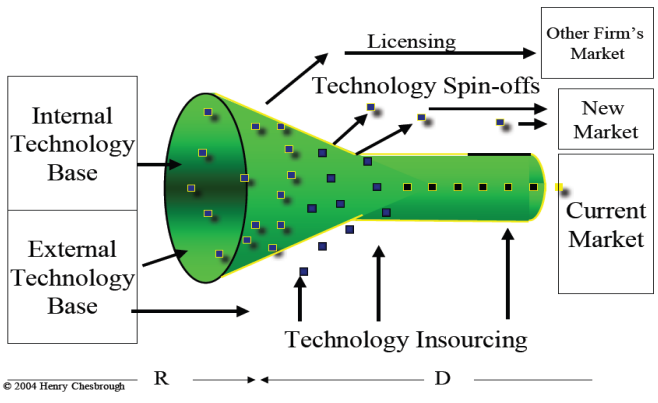
\includegraphics[width=0.8\textwidth]{images/open.png}
\end{figure}
\FloatBarrier
\subparagraph{Chiuso}
\begin{itemize}
    \item Progetti lanciati da basi tecnolgiche/scientifiche esclusivamente interne
    \item Selezione specifica di progetti che possono continuare il processo
    \item Solo alcuni progetti vanno sul mercato
\end{itemize}
\FloatBarrier
\begin{figure}[!htb]
    \centering
    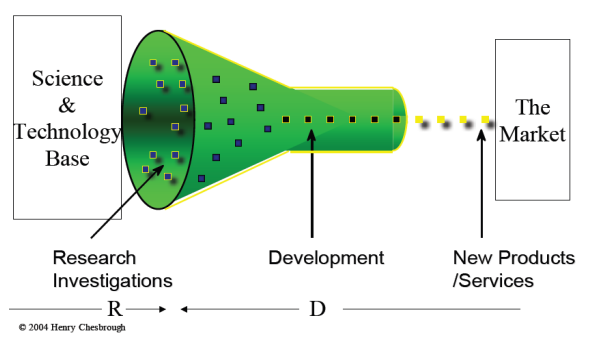
\includegraphics[width=0.8\textwidth]{images/closed.png}
\end{figure}
\FloatBarrier
\newpage
\subsection{Venture Capital e finanziamento di aziende di start up e spin-off: in cosa si differenzia rispetto ai canali normali di finanziamento?}
Investimento di medio/lungo periodo. L’investitore decide di puntare su società definite “high grow companies”, ossia ad alto potenziale di crescita e sviluppo, nel momento in cui esse sono però ancora agli esordi.
L’obiettivo del venture capital è quello di finanziare la società, farla crescere e poi ottenere un guadagno dalla vendita della propria partecipazione o comunque dalla quotazione in Borsa della stessa azienda. Nonostante i rischi per l’investitore siano elevati, le possibilità di guadagno derivanti dal successo della start up sono molto attraenti.\\
I normali istituti di credito fungono da veicolo per finanziamenti e sono soliti anche richiedere interessi dopo un prestito. I venture capital sono invece quote destinate a investimenti diretti operati da un venture capitalist che ha interesse nel guadagno dalla crescita della startup, quindi solitamente non richiede garanzie e non prevede interessi.
\newpage
\subsection{Classificazione tra piccole, medie e grandi imprese}
\FloatBarrier
\begin{figure}[!htb]
    \centering
    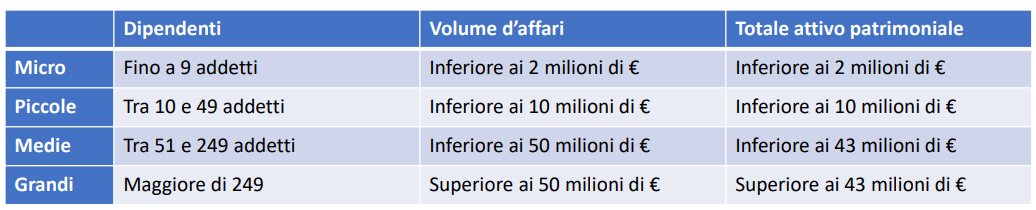
\includegraphics[width=1\textwidth]{images/pmi.png}
\end{figure}
\FloatBarrier
\newpage
\subsection{Immobilizzazioni materiali e immateriali ed i relativi ammortamenti: quali possono essere i criteri di valutazione delle immateriali?}
Immobilizzazioni immateriali: marchi e brevetti, hanno un costo, proteggono la proprietà intellettuale, ma al tempo stesso la divulgano. Il valore di un’azienda è influenzato in modo positivo dalla presenza di asset immateriali. I progetti di innovazione presentano rischi particolari e utilizzano strumenti specifici per la loro mitigazione.\\
Immobilizzazioni immateriali nello \textbf{stato patrimoniale} relativi alla voce \textbf{attivo}.
Il conto economico deve riportare come costi di ammortamento la svalutazione annuale dell’immobilizzazione.
\\Criteri di valutazione \textbf{discrezionali}:
\begin{itemize}
    \item Disponibilità temporale
    \item Proprietà
    \item Unicità
\end{itemize}

La quota di ammortamento annua di ciascuna categoria di immobilizzazioni viene inserita tra i costi del conto economico, e contemporaneamente, contribuisce al formarsi di un fondo ammortamento, posto a rettifica del valore del bene cui si riferisce nello stato patrimoniale.
Il valore contabile dell’immobilizzazione è progressivamente ridotto da questo processo: in bilancio (attivo dello stato patrimoniale) compare il valore contabile del bene al netto dell’ammortamento cumulato.

\newpage
\subsection{Come un'azienda acquisisce i mezzi finanziari: azioni, obbligazioni e prestiti bancari. Caratteristiche, vantaggi e svantaggi}
\paragraph{Azioni}
Strumenti finanziari con un valore negoziabili. Vengono messe sul mercato dalle aziende per aumentarne il capitale sociale.
\subparagraph{Pro}
\begin{itemize}
    \item Voto nelle assemblee
    \item Controllo della gestione
    \item Partecipazione ai dividendi
\end{itemize}
\subparagraph{Contro}
\begin{itemize}
    \item Non garantiscono il ritorno del capitale investito
\end{itemize}
\paragraph{Obbligazioni}
Le obbligazioni sono prestiti che verranno rimborsati e che garantiscono un interesse. Acquistare un’obbligazione vuol dire prestare soldi a un’azienda, a una banca, a uno Stato o a un ente pubblico, e diventare creditori verso uno di questi “emittenti” e poter vantare il diritto alla restituzione di quanto è stato prestato e di una somma in più, gli interessi, come compenso per aver prestato quel denaro.
\subparagraph{Pro}
\begin{itemize}
    \item Danno diritto alla restituzione del capitale più l'interesse
\end{itemize}
\subparagraph{Contro}
\begin{itemize}
    \item Basate sull'affidabilità del debitore
    \item Soldi impegnati per un lasso di tempo predeterminato
\end{itemize}
\paragraph{Prestiti Bancari}
Forme di finanziamento erogate da istituti di credito che prevedono la restituzione del capitale più interessi
\subparagraph{Pro}
\begin{itemize}
    \item Solidità dell'ente creditore
\end{itemize}
\subparagraph{Contro}
\begin{itemize}
    \item Tempi e modalità di accesso complessi
    \item Spread
\end{itemize}
\subsection{Quali sono i vantaggi e gli svantaggi per un'azienda a seguito della quotazione in borsa?}
Una parte più o meno ampia del capitale di rischio anziché essere detenuta in modo stabile da una persona (o gruppo) è soggetta a una sistematica compravendita sul mercato. Tramite la borsa valori, qualsiasi risparmiatore privato o intermediario finanziario può acquisire azioni di quell’impresa divenendo così parte del suo soggetto economico.
\paragraph{Contro}
\begin{itemize}
    \item Soggetto economico molto frammentato
    \item Potenzialmente controllabili da soci di minoranza particolarmente organizzati
    \item La quotazione in borsa impone alle aziende obblighi particolari per la gestione (relazione trimestrale sull’andamento)
\end{itemize}
\paragraph{Pro}
\begin{itemize}
    \item Aumento del capitale sociale
    \item Attrazione di investitori esterni
\end{itemize}
\subsection{Cosa si intende per valore attualizzato, valore attualizzato netto e tasso interno di rendimento?}
\paragraph{VA (Valore Attuale)} di una successione di flusso di cassa con tasso $r$ è $$VA = {x_0+{x_1\over(1+r)^1}+{x_2\over(1+r)^2}+\dots+{x_n\over(1+r)^n}}$$
dove $x_i$ è flusso di cassa $x$ a tempo $i$
\paragraph{VAN (Valore Attualizzato netto)}  Valore attualizzato delle entrate e uscite - investimento iniziale. Calcolato il VAN si può valutare l’investimento in questo modo:
\begin{itemize}
    \item Accettare se $VAN > 0$ perché indica che il rendimento futuro è superiore al costo opportunità del capitale investito.
    \item Rifiutare se $VAN<0$ perché il rendimento futuro è inferiore al costo opportunità del capitale investito.
\end{itemize}
\paragraph{TIR (Tasso Interno di Rendimento)} Misura del bilancio del capitale, viene utilizzato dalle società per determinare la redditività di un potenziale investimento o progetto sul flusso di cassa previsto
\newpage
\subsection{Cosa sono le curve di domanda/offerta e determinazione del prezzo di equilibrio?}
\paragraph{Curva di offerta} \textit{Relazione tra la quantità di un bene che i produttori sono disposti a vendere e il prezzo del bene}. Questa curva è inclinata positivamente: maggiore è il prezzo, più imprese possono e desiderano produrre e vendere. Variabile che influenza l'offerta è relativa ai \textbf{costi di produzione}, che comprendono i salari, gli interessi passivi sui capitali investiti, il costo delle materie prime e di eventuali licenze. Quando i costi di produzione diminuiscono, la produzione aumenta indipendentemente dal prezzo di mercato. L’intera curva di offerta si sposta quindi verso destra
\FloatBarrier
\begin{figure}[!htb]
    \centering
    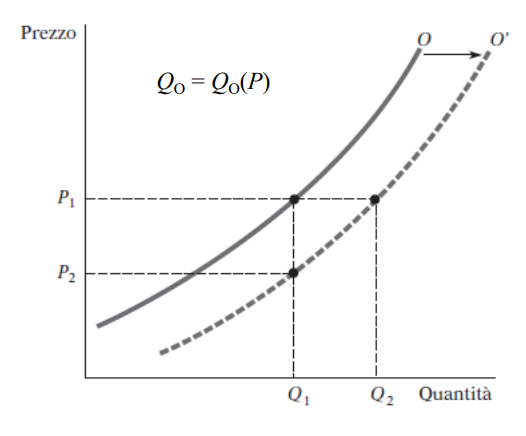
\includegraphics[width=1\textwidth]{images/offerta.png}
    \caption{Curva di Offerta}
\end{figure}
\paragraph{Curva di Domanda}
\textit{Relazione tra la quantità di un bene che i consumatori sono disposti ad acquistare e il prezzo del bene}. Questa curva è inclinata negativamente: mantenendo costanti gli altri fattori, i consumatori saranno disposti ad acquistare maggiori quantità di un bene quando il
prezzo di quest’ultimo diminuisce. La quantità domandata può dipendere anche da altre variabili, come il reddito, il clima e i prezzi di altri beni. Per la maggior parte dei prodotti, la quantità domandata aumenta al diminuire del prezzo.
\FloatBarrier
\begin{figure}[!htb]
    \centering
    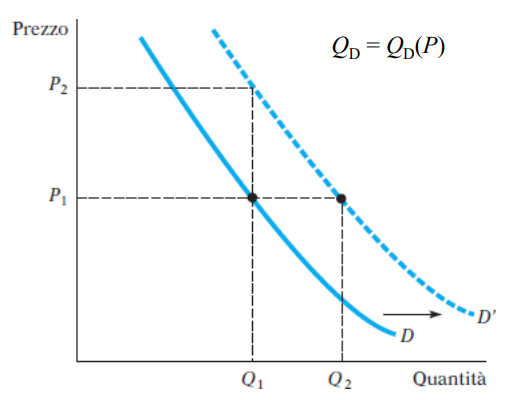
\includegraphics[width=1\textwidth]{images/domanda.png}
    \caption{Curva di Domanda}
\end{figure}
\paragraph{Meccanismo di Mercato}
\begin{itemize}
    \item Il mercato è in equilibrio al prezzo $P_0$ e alla quantità $Q_0$.
    \item Al prezzo più alto $P_1$ si sviluppa un’eccedenza, che fa diminuire il prezzo.
    \item Al prezzo più basso $P_2$ si determina una scarsità, che fa aumentare il prezzo.
\end{itemize}
\FloatBarrier
\begin{figure}[!htb]
    \centering
    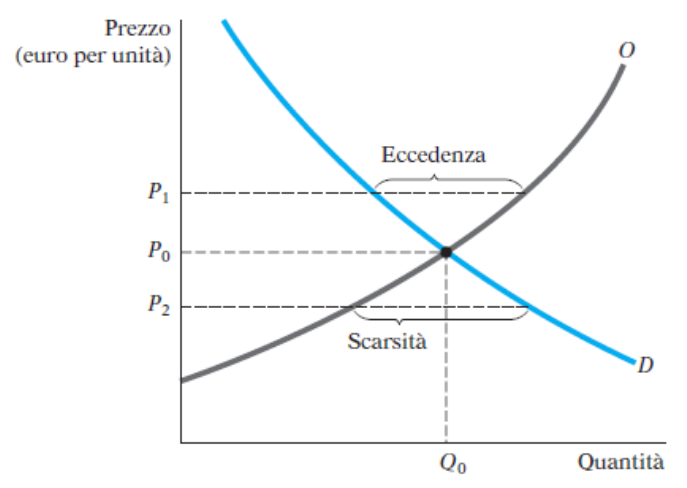
\includegraphics[width=1\textwidth]{images/mercato.png}
    \caption{Meccanismo di Mercato}
\end{figure}
\begin{itemize}
    \item \textbf{Prezzo di equilibrio} Prezzo al quale la quantità domandata e la quantità offerta si equivalgono.
    \item \textbf{Meccanismo di mercato} Nei mercati liberi, tendenza del prezzo a variare fino a quando quantità domandata e quantità offerta si equivalgono.
    \item \textbf{Eccedenza} Situazione in cui la quantità offerta supera la quantità domandata.
    \item \textbf{Scarsità} Situazione in cui la quantità domandata supera la quantità offerta.
\end{itemize}
\newpage
\subsection{Cosa si intende per elasticità della domanda rispetto al prezzo?}
L’elasticità della domanda rispetto al prezzo indica quanto la domanda di determinati beni o servizi sia sensibile alle variazioni di prezzo.\\
Normalmente, un aumento dei prezzi porta ad un calo della domanda perché i consumatori non possono o non vogliono spendere più soldi per il prodotto o servizio in questione. Al contrario, una riduzione dei prezzi porta ad un aumento della domanda. In questi casi si parla di domanda elastica rispetto al prezzo, poiché dipende fortemente dal prezzo e può oscillare in base ad esso.
$$E_p={\% \Delta Q \over{\% \Delta P }}$$

\newpage
\subsection{Incertezza e comportamento del consumatore: cos'è e come si rappresenta la propensione al rischio?}
Descrizione del rischio
\begin{itemize}
    \item Probabilità: Probabilità che si verifichi un certo evento
    \item Valore atteso: Media ponderata dei payoff associati ai possibili esiti, calcolata utilizzando come pesi le probabilità degli esiti
    \item Payoff: Valore associato a un possibile esito
\end{itemize}
La propensione al rischio viene misurata mediante payoff in termini di \textbf{utilità} invece che in termini monetari. L’utilità è una funzione
monotona crescente della variabile monetaria.
\paragraph{Utilità attesa} Somma delle utilità associate a tutti i possibili esiti, pesate dalle probabilità
che i rispettivi esiti si verifichino.
\begin{itemize}
    \item \textbf{Propensione al rischio}: preferenza per un reddito incerto rispetto a un reddito certo avente lo stesso valore atteso. $D'' > 0$
    \item \textbf{Avversione al rischio}: preferenza per un reddito certo rispetto a un reddito rischioso avente lo stesso valore atteso. $D'' < 0$
    \item \textbf{Neutralità al rischio}: indifferenza tra un reddito certo e un reddito incerto aventi lo stesso valore atteso. $f$ lineare
\end{itemize}
Per ridurre il rischio occorre "comprare" informazioni aggiuntive
\newpage
\subsection{Recommender System}
Un sistema di raccomandazioni utilizza dati di diverso tipo forniti da utenti per raggiungere obiettivi di:
\begin{itemize}
    \item \textbf{Rilevanza}: raccomandare prodotti che un utente ritiene più interessanti
    \item \textbf{Novità}: raccomandare prodotti che un utente potrebbe non avere ancora visto
    \item \textbf{Serendipitività}: suggerire prodotti "inaspettati" ma che potrebbero piacere all'utente
    \item \textbf{Incremento della diversità}: Suggerire prodotti di "diverso" tipo per non annoiare l'utente
\end{itemize}
I rating sono valutazioni lasciate dagli utenti e possono essere:
\begin{itemize}
    \item a valori continui (anche se raro)
    \item a valori interi in uno specifico intervallo (ad esempio una scala formata da 5 rating, 1-5)
    \item a valori categorici (fortemente d’accordo, d’accordo, in disaccordo, fortemente in disaccordo, neutro)
    \item a valori binari (0/1, -1/+1,dislike/like)
    \item a valori unari (1 se mi piace come in Facebook)
\end{itemize}
Le matrici di rating presentano in una dimensione l'utente e nell'altra il relativo item a cui viene dato il rating che si troverà nell'intersezione di riga e colonna. Le matrici di rating potrebbero non rappresentare del tutto le informazioni relative ad un utente. \\Per questo a volte occorre far uso di rating di tipo implicito (es. durata di visione di un film etc.). Un recommender system può essere di conseguenza valutato mediante diversi criteri tra cui l'accuracy che prevede
\begin{itemize}
    \item Predizione del rating
    \item Predizione del ranking
\end{itemize}
Le entrate vuote della matrice possono essere completate mediante l'utilizzo di metodi
\begin{itemize}
    \item \textbf{Collaborative Filtering (basati sul concetto di community)} PRO E CONTRO
          \begin{itemize}
              \item \textit{Memory-Based (neighbourhood similarity k-NN)} PRO E CONTRO
              \item \textit{Model-Based} PRO E CONTRO
          \end{itemize}
    \item \textbf{Content-Based} PRO E CONTRO
\end{itemize}
\newpage
\subsection{Misure di similarità: coseno e pearson}
La cosine similarity rappresenta una misura di somiglianza tra 2 vettori.
Geometricamente corrisponde al coseno dell’angolo tra i due vettori. Nel caso in cui le componenti dei vettori siano non-negative (come nel caso
dei ratings), la cosine similarity può variare tra 0 (completa diversità) a +1 (massima somiglianza). È invariante rispetto alle dilatazioni. La cosine similarity può essere definita anche nel caso in cui non siano note alcune componenti dei due vettori: per farlo si considera l’insieme $I_{ab}$ come l’insieme degli indici delle componenti note sia di $a$ che di $b$, e si definisce la cosine similarity come la somma dei prodotti scalari diviso la somma dei prodotti tra i moduli
$$sim(\vec{a}, \vec{b}) = {{\vec{a} \cdot \vec{b}}\over{||\vec{a}|| \cdot ||\vec{b}||}}$$
\begin{itemize}
    \item $\Theta = {\pi \over 2}$ completa diversità
    \item $\Theta = 0$ massima somiglianza
\end{itemize}
Un'altra misura di similarità è data dall’indice di correlazione di Pearson
$$sim(\vec{a}, \vec{b}) = {{\sum_{i=1}^{n}{(a_i - \overline{a}) \cdot (b_i - \overline{b})}}\over{||\vec{a}|| \cdot ||\vec{b}||}}$$
\newpage
\subsection{Cosa si intende per k-NN}
Il modo più semplice per definire un neighborhood di uno target user consiste nel considerare l’insieme di $k$ users con l’indice di similarità (cosine o pearson) più alto. Una volta calcolato il neighbourhood per un target user per un item specifico, si può procedere a calcolare il rating predetto per tale item come media dei rating appartenenti al neighborhood relativo.
Abbiamo usato k-NN per effettuare «regressione» arrivare cioè a una stima con un valore continuo, che possiamo poi associare a una variabili discreta.
\\Per determinare un opportuno vicino di uno user/item è necessario stabilire:
\begin{itemize}
    \item un’opportuna misura di similarità
    \item il numero di vicini $k$ è da considerare un iperparametro
    \item Come si determinano queste scelte ? Automated machine learning (AutoML)
\end{itemize}
Cerchi per k diverse e due classi con elemento centrale da classificare.
\newpage
\subsection{Cosa sono training e test set?}
\begin{itemize}
    \item Un generico algoritmo di Machine Learning supervisionato utilizza i dati del training set per simulare la conoscenza pregressa ed approssimare la funzione
    \item Utilizza i dati del test set per confrontare i risultati del modello appreso (trained) con risultati “veri” non usati nell’addestramento del modello e calcolare una misura di accuratezza dell’algoritmo di machine learning
\end{itemize}
Dividere l’insieme dei dati in training set e test contiene un elemento di distorsione e quindi non essere sufficiente per
un loro bilanciamento significativo. Per ottenere questo un modo è utilizzare la cross-validation.
\begin{enumerate}
    \item Si divide il dataset in $k$ gruppi apprrossimativamente della stessa dimensione
    \item Si valuta $k$ volte l’accuratezza usando un gruppo per il test set e gli altre $k-1$ gruppi come training set
    \item Si ottiene un campione di $k$ misure di accuratezza e se ne considera la media come stimatore. Varianza si riduce all’aumentare di $k$
\end{enumerate}
\begin{itemize}
    \item vantaggi: in questo modo utilizziamo tutti i dati del dataset k volte
    \item svantaggi: richiede più tempo, andrebbe ripetuta per diversi valori di iperparametri
\end{itemize}
Nel dataset la divisione tra training e test deve essere bilanciata.
Una misura di accuratezza potrebbe essere la media delle differenze in modulo tra la previsione basata sul training e le osservazioni presenti nel test set.
\newpage
\subsection{Problemi di Classificazione: cosa significano TP, FP, TN e FN e come si possono costruire su di essi gli indici di precisione e di recall}
Nei problemi di classificazione, l’obiettivo della predizione è quello di riconoscere a quale tra 2 o più classi un elemento appartiene.
\\Un algoritmo di classificazione può essere valutato attraverso l’utilizzo della matrice di confusione. Essa corrisponde ad una
tabella di 4 differenti possibili combinazioni tra valori predetti e valori veri (positivo-like , negativo-dislike)
\begin{itemize}
    \item TP (Veri positivi): predico 1, ed il valore vero è 1
    \item FP (Falsi positivi): predico 1, ed il valore vero è 0
    \item TN (Veri negativi): predico 0, ed il valore vero è 0
    \item FN (Falsi negativi): predico 0, ed il valore vero è 1
\end{itemize}
Per misurare la correttezza della predizione per una matrice di rating binaria è possibile utilizzare la matrice di confusione.
Dove:
\begin{itemize}
    \item TP è il numero \% di item correttamente classificati come like
    \item FP numero \% gli item classificati come like MA in realtà sono dislike
    \item TN per gli item classificati come dislike e che sono dislike
    \item FN per gli item classificati come dislike MA che in realtà sono like
\end{itemize}

Nel caso ideale vorrei che la matrice di confusione fosse diagonale.
Se FP=FN=0 allora le mia classificazione è perfettamente corretta (TP=TN=1).
Dalla matrice di confusione è possibile estrarre le misure di Precision e Recall

$$P = {item \ raccomandati \ correttamente \over item \ totali} = {TP \over {TP + FP}}$$
$$R = {item \ raccomandati \ correttamente \over item \ raccomandati}= {TP \over {TP + FN}}$$
Precision e recall sono misure «antagoniste», un'alta precisione implica una bassa recall e viceversa.
Tali misure possono essere poi studiate in funzione di un parametro $\tau$.\\
Essendo l’output del k-NN un valore continuo tra 0 e 1 è possibile fissare un valore di threshold $\tau$.\\
Al variare del parametro di soglia $\tau$ possiamo avere performance diverse per l’algoritmo

\end{document}

